\usepackage{amsmath,amssymb,amsthm}
\usepackage[all]{xy}
\usepackage{graphicx}
\usepackage[backend=biber,style=alphabetic,maxnames=99,giveninits=true,url=false,isbn=false]{biblatex}
\addbibresource{refs.bib}



\numberwithin{equation}{subsection}

% Basic macros
\def\lim{\mathop{\mathrm{lim}}\nolimits}
\def\colim{\mathop{\mathrm{colim}}\nolimits}
\def\Spec{\mathop{\mathrm{Spec}}}
\def\Hom{\mathop{\mathrm{Hom}}\nolimits}
\def\Ext{\mathop{\mathrm{Ext}}\nolimits}
\def\Ker{\mathop{\mathrm{Ker}}}
\def\Im{\mathop{\mathrm{Im}}}
\def\Coker{\mathop{\mathrm{Coker}}}
 \def\Coim{\mathop{\mathrm{Coim}}}

% Slide numbering
\addtobeamertemplate{navigation symbols}{}{%
    \usebeamerfont{footline}%
    \usebeamercolor[fg]{footline}%
    \hspace{1em}%
    \insertframenumber/\inserttotalframenumber
}


\title{Deformations of Stanley--Reisner schemes}
\subtitle{Smoothing the Grünbaum sphere}
\date{Informal talk, PUC-Rio \quad 3 December 2026}
% Divider for the seven parts: number, title, what the part does.
\usepackage{array}
\newcommand{\partslide}[3]{\begin{frame}\centering
{\large Part #1}\par\medskip{\huge #2\par}\par\vspace{6mm}
\begin{minipage}{0.78\textwidth}\centering #3\end{minipage}\end{frame}}
% The link of b, drawn flat (the picture of Part 2), at a given scale.
\newcommand{\linkofb}[1]{\begin{tikzpicture}[scale=#1,line join=round]
\coordinate (g) at (0,3.3);
\coordinate (f) at (-3.7,-2.3);
\coordinate (h) at (3.7,-2.3);
\coordinate (c) at (0,1.3);
\coordinate (e) at (-1.3,-1.2);
\coordinate (d) at (0.9,-0.9);
\coordinate (a) at (-0.13,-0.27);
\draw (f)--(g)--(h)--cycle;
\draw (c)--(f) (c)--(g) (c)--(h) (c)--(e) (c)--(d) (c)--(a);
\draw (e)--(f) (d)--(h) (d)--(e) (a)--(d) (a)--(e) (e)--(h);
\foreach \p/\pos in {g/above,f/below left,h/below right,c/above right,e/below left,d/right,a/below}
  \fill (\p) circle (1.5pt) node[\pos]{\(\p\)};
\end{tikzpicture}}
\begin{document}
\begin{frame}\titlepage
\vfill\centering{\footnotesize\href{https://www.heap-project.org/talks/stanley-reisner-puc-informal/live.html}{\textcolor{blue}{Click here for the live version}} (slides with moving models)}
\end{frame}

\partslide{1}{What I will do}{The main theorem, and the main steps of its proof.}

\begin{frame}{The main theorem}
\begin{columns}[c]
\begin{column}{0.64\textwidth}
\textbf{Deformation.} Let \(X\) be a scheme. A \emph{deformation} of \(X\) is a Cartesian diagram as on the right, where \(\pi\) is a flat surjective morphism of algebraic \(\C\)-schemes and \(B\) is connected.
\par\medskip
\textbf{Smoothing.} A deformation where the general fibre \(X_t\) of \(\pi\) is smooth.
\end{column}
\begin{column}{0.32\textwidth}\centering
\begin{tikzpicture}[>=Stealth]
\node (X) at (0,1.5) {\(X\)};
\node (XX) at (2.4,1.5) {\(\mathcal X\)};
\node (pt) at (0,0) {\(\operatorname{Spec}\C\)};
\node (B) at (2.4,0) {\(B\)};
\draw[->] (X)--(XX);
\draw[->] (X)--(pt);
\draw[->] (XX)--node[right]{\(\pi\)}(B);
\draw[->] (pt)--(B);
\end{tikzpicture}
\end{column}
\end{columns}
\par\medskip
\textbf{The sphere.} \(\mathcal M\): a triangulation of the \(3\)-sphere with \(8\) vertices and \(20\) tetrahedra \cite{GS}.
\par\medskip
\textbf{The scheme.} \(X=\SR(\mathcal M)\subset\Pj^7\): one \(\Pj^3\) for each tetrahedron, glued as the tetrahedra are glued.
\par\medskip
\fbox{\begin{minipage}{0.96\linewidth}
\textbf{Theorem (proposed).} \(X\) has a smoothing over a curve, in which every fibre other than \(X\) is a smooth Calabi--Yau threefold of degree \(20\) in \(\Pj^7\).
\end{minipage}}
\src{\textbf{Status.} The proof was assembled with AI help and checked by an AI audit. I am verifying it by hand; this is not finished.}
\end{frame}


\begin{frame}{The proof in three steps}
\begin{center}
\begin{tikzpicture}[>=Stealth,box/.style={draw,rounded corners=2pt,align=center,inner sep=4pt,font=\small}]
\node[box] (a) at (0,0) {\(\SR(\mathcal M)\)\\ sixteen cubics};
\node[box] (b) at (3.6,0) {formal family\\ over \(\C[[t]]\)};
\node[box] (c) at (7.2,0) {its generic fibre\\ is smooth};
\node[box] (d) at (10.8,0) {family over\\ a curve \(C\)};
\draw[->] (a)--node[above]{\small 1}(b);
\draw[->] (b)--node[above]{\small 2}(c);
\draw[->] (c)--node[above]{\small 3}(d);
\end{tikzpicture}
\end{center}
\begin{enumerate}
\setlength{\itemsep}{4pt}
\item \textbf{A formal family} (Parts 4 and 5). \(\mathcal M\) has a group of symmetries \(G\simeq S_3\). A \(G\)-equivariant first-order deformation extends to all orders in \(t\).
\item \textbf{Its generic fibre is smooth} (Part 6). By contradiction. A singular point would come down to a point of \(\SR(\mathcal M)\), in some face of \(\mathcal M\). Shown for one face, the triangle \(beh\).
\item \textbf{Algebraization} (Part 7). The power series in \(t\) are replaced by a family over a curve.
\end{enumerate}
\textbf{The smooth fibres are then Calabi--Yau} (Part 3): this holds for every triangulated \(3\)-sphere. Not proved.
\end{frame}

\partslide{2}{What is \(\mathcal M\)?}{Pictures of \(\mathcal M\), to get used to it. They are not needed for the proof.}

\begin{frame}{Spheres made of simplices}
\textbf{Definition.} A \emph{triangulated \(d\)-sphere}: simplices of dimension \(d\), glued along their faces, so that the result is topologically the sphere \(S^d\).
\par\medskip
\begin{columns}[t]
\begin{column}{0.3\textwidth}
\centering
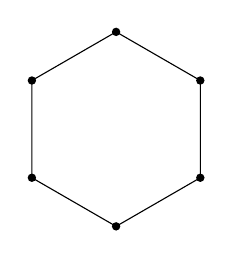
\begin{tikzpicture}[scale=0.95]
\foreach \i in {0,...,5} \coordinate (p\i) at ({90+60*\i}:1.3);
\draw (p0)--(p1)--(p2)--(p3)--(p4)--(p5)--cycle;
\foreach \i in {0,...,5} \fill (p\i) circle (1.6pt);
\end{tikzpicture}
\par\medskip
\textbf{A circle.}\\ 6 vertices, 6 edges.
\end{column}
\begin{column}{0.3\textwidth}
\centering
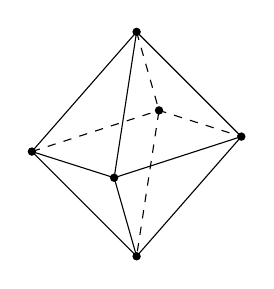
\begin{tikzpicture}[scale=0.95,line join=round]
\coordinate (t) at (0,1.5); \coordinate (u) at (0,-1.5);
\coordinate (w) at (-1.4,-0.1); \coordinate (x) at (-0.3,-0.45);
\coordinate (y) at (1.4,0.1); \coordinate (z) at (0.3,0.45);
\draw[dashed] (w)--(z)--(y) (t)--(z)--(u);
\draw (w)--(x)--(y) (t)--(w)--(u) (t)--(x)--(u) (t)--(y)--(u);
\foreach \p in {t,u,w,x,y,z} \fill (\p) circle (1.6pt);
\end{tikzpicture}
\par\medskip
\textbf{A \(2\)-sphere.}\\ 6 vertices, 12 edges, 8 triangles.
\end{column}
\begin{column}{0.36\textwidth}
\centering
\vspace{8mm}
{\Huge \(\mathcal M\)}
\par\vspace{6mm}
\textbf{A \(3\)-sphere.}\\ 8 vertices, 28 edges, 40 triangles, 20 tetrahedra.
\end{column}
\end{columns}
\src{\textcolor{red}{I did not confirm the incidence relations in any picture of this talk.}}
\end{frame}

\begin{frame}{The link of a vertex}
The \emph{link} (or vertex figure) of a vertex: what is at incidence distance \(1\) from it.
\begin{columns}[c]
\begin{column}{0.5\textwidth}\centering
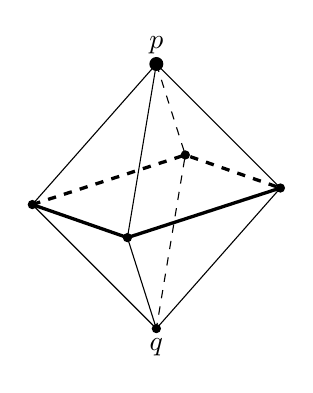
\begin{tikzpicture}[scale=1.05,line join=round]
\coordinate (t) at (0,1.6); \coordinate (u) at (0,-1.6);
\coordinate (w) at (-1.5,-0.1); \coordinate (x) at (-0.35,-0.5);
\coordinate (y) at (1.5,0.1); \coordinate (z) at (0.35,0.5);
\draw[dashed] (t)--(z)--(u);
\draw (t)--(w)--(u) (t)--(x)--(u) (t)--(y)--(u);
\draw[very thick,dashed] (w)--(z)--(y);
\draw[very thick] (w)--(x)--(y);
\foreach \p in {u,w,x,y,z} \fill (\p) circle (1.6pt);
\fill (t) circle (2.4pt) node[above]{\(p\)};
\node[below] at (u) {\(q\)};
\end{tikzpicture}
\par\smallskip
\textbf{The octahedron.} The link of \(p\) is the thick square. The vertex \(q\) is at distance \(2\): it is not in the link.
\end{column}
\begin{column}{0.48\textwidth}\centering
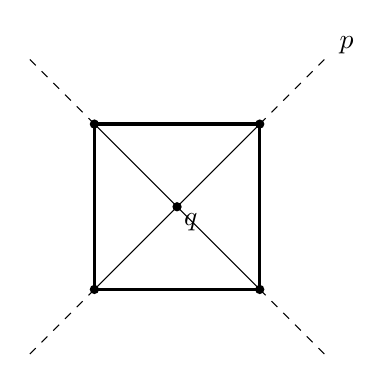
\begin{tikzpicture}[scale=1.05,line join=round]
\foreach \a/\b/\n in {-1/-1/A,1/-1/B,1/1/C,-1/1/D} \coordinate (\n) at (\a,\b);
\coordinate (q) at (0,0);
\foreach \n/\a/\b in {A/-1/-1,B/1/-1,C/1/1,D/-1/1} \draw[dashed] (\n)--++(0.8*\a,0.8*\b);
\draw (q)--(A) (q)--(B) (q)--(C) (q)--(D);
\draw[very thick] (A)--(B)--(C)--(D)--cycle;
\foreach \n in {A,B,C,D} \fill (\n) circle (1.6pt);
\fill (q) circle (1.6pt) node[below right=-1pt]{\(q\)};
\node at (2.05,1.95) {\(p\)};
\end{tikzpicture}
\par\smallskip
\textbf{The same, seen from \(p\).} Inside the square: the \(4\) triangles that do not touch \(p\). Outside: the \(4\) triangles at \(p\); the dashed edges go to \(p\), which is at infinity.
\end{column}
\end{columns}
\end{frame}

\begin{frame}{\(\mathcal M\) seen from a vertex}
\vspace{2mm}
\begin{columns}[t]
\begin{column}{0.46\textwidth}\centering
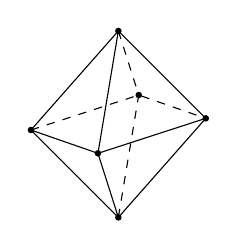
\begin{tikzpicture}[scale=0.74,line join=round]
\coordinate (t) at (0,1.6); \coordinate (u) at (0,-1.6);
\coordinate (w) at (-1.5,-0.1); \coordinate (x) at (-0.35,-0.5);
\coordinate (y) at (1.5,0.1); \coordinate (z) at (0.35,0.5);
\draw[dashed] (t)--(z)--(u) (w)--(z)--(y);
\draw (t)--(w)--(u) (t)--(x)--(u) (t)--(y)--(u) (w)--(x)--(y);
\foreach \p in {t,u,w,x,y,z} \fill (\p) circle (1.6pt);
\end{tikzpicture}
\par\smallskip
\textbf{The \(16\)-cell}: a regular \(3\)-sphere with \(8\) vertices and \(16\) tetrahedra.
\par\smallskip
The link of a vertex is an octahedron: \(6\) of the \(7\) other vertices. Inside it: the \(8\) tetrahedra that do not touch the vertex.
\par\smallskip
All \(8\) vertices look the same: \(384\) symmetries.
\end{column}
\begin{column}{0.52\textwidth}\centering
\linkofb{0.4}
\par\smallskip
\textbf{\(\mathcal M\)}: \(8\) vertices and \(20\) tetrahedra.
\par\smallskip
The link of \(b\), drawn flat: all \(7\) other vertices, \(10\) triangles. Inside it: the \(10\) tetrahedra that do not touch \(b\).
\par\smallskip
The vertices do not all look the same: the links of \(d\) and \(f\) are different from the other six. Only \(6\) symmetries (Part 4).
\end{column}
\end{columns}
\end{frame}





\begin{frame}{\(\mathcal M\) is a non-polytopal sphere}
\textbf{Definition.} A simplicial \(d\)-sphere is \emph{polytopal} if it is isomorphic to the boundary of a convex simplicial \((d+1)\)-polytope.
\par\smallskip
To prove non-polytopality, every possible convex realization must be ruled out. A nonconvex drawing proves nothing.
\par\smallskip
\textbf{Where it starts.} Every simplicial \(2\)-sphere is polytopal (Steinitz). Non-polytopal spheres start in dimension \(3\).
\par\smallskip
\textbf{Our sphere.} Grünbaum--Sreedharan \cite{GS}, Theorem 2: \(\mathcal M\), with \(8\) vertices and \(20\) tetrahedra, is not the boundary of any \(4\)-polytope.
\par\medskip
\textbf{Among \(8\)-vertex \(3\)-spheres.} There are \(39\) types; \(37\) are polytopal and two are not: \(\mathcal M\) and Barnette's sphere.
\par\medskip
\textbf{For this talk.} Non-polytopality is not, by itself, an obstruction to smoothing \(\SR(\mathcal M)\).
\src{The count of \(8\)-vertex spheres is Barnette (1973), cited from my notes, not re-read.}
\end{frame}

\begin{frame}{Basic information about \(\mathcal M\)}
\textbf{What it is.} A triangulation of the \(3\)-sphere with \(8\) vertices \(a,\dots,h\), which is not the boundary of a \(4\)-polytope \cite{GS}.
\par\medskip
\textbf{Counts.} \(8\) vertices, \(28\) edges, \(40\) triangles, \(20\) tetrahedra. Every two vertices are joined by an edge.
\par\medskip
\textbf{The \(16\) triples that are not triangles} (the sixteen cubics):
\[
abf,\ abg,\ abh,\ acg,\ ach,\ adh,\ bdf,\ bdg,\ beg,\ cde,\ ceg,\ ceh,\ cfh,\ def,\ dfh,\ efg.
\]
\textbf{The Stanley--Reisner ideal.} In \(\C[a,\dots,h]\), one variable per vertex, a set of vertices \(S\) gives the monomial \(x_S=\prod_{i\in S}x_i\). The ideal \(I_{\mathcal M}\) is generated by the \(x_S\) for the sets \(S\) that are not faces of \(\mathcal M\). Here it is generated by the sixteen cubics above.
\end{frame}

\partslide{3}{Why Calabi--Yau, and motivation}{Why a smoothing of the scheme of a triangulated \(3\)-sphere is a Calabi--Yau threefold: the scheme of a sphere has a trivial dualizing sheaf, and this passes to a smoothing. After that: why we look at \(\mathcal M\).}

\begin{frame}{A smoothing of a sphere is Calabi--Yau}
\textbf{Setting.} A triangulated \(3\)-sphere \(\Delta\) with \(n\) vertices. Its ring \(R=\C[x_1,\dots,x_n]/I_\Delta\) and its scheme \(X=\Proj R\subset\Pj^{n-1}\): one \(\Pj^3\) for each tetrahedron, glued as the tetrahedra are. A smoothing: a flat projective family over a curve, with fibre \(X\) over \(0\) and smooth fibres \(Y\) nearby.
\par\medskip
\textbf{Statement.} \(K_Y\simeq\cO_Y\) and \(H^1(\cO_Y)=H^2(\cO_Y)=0\): \(Y\) is a Calabi--Yau threefold.
\par\medskip
\textbf{What replaces \(K\) on \(X\).} \(X\) is singular, so it has no bundle of \(3\)-forms. It has a dualizing sheaf \(\omega_X\): the sheaf that takes the place of \(K\) in Serre duality. On a smooth variety, \(\omega=K\).
\par\medskip
\textbf{The proof has two halves.}
\begin{enumerate}
\setlength{\itemsep}{2pt}
\item \emph{On \(X\): combinatorics.} \(\omega_X\simeq\cO_X\). The reason: \(\Delta\) is a sphere.
\item \emph{From \(X\) to \(Y\): deformation theory.} A trivial \(\omega_X\), together with \(H^1(X,\cO_X)=0\), passes to the nearby fibres.
\end{enumerate}
\end{frame}

\begin{frame}{The links of a sphere are spheres}
\textbf{Link.} For a face \(\sigma\) of \(\Delta\): \(\ \operatorname{lk}\sigma=\{\tau\in\Delta:\ \tau\cap\sigma=\varnothing,\ \tau\cup\sigma\in\Delta\}\).
\par\smallskip
\textbf{In a triangulated \(3\)-sphere.} The link of a vertex is a \(2\)-sphere. Of an edge: a circle. Of a triangle: two points. Of the empty face: \(\Delta\) itself. Always a sphere, of dimension \(3-|\sigma|\).
\par\smallskip
\textbf{Reisner, Stanley.} If every link has the homology of a sphere of its dimension, then \(R\) is Gorenstein and \(\ \boxed{\omega_R\simeq R}\ \) as graded modules, with no shift.
\par\smallskip
\textbf{Where the sphere enters (idea, not proof).} Take a monomial whose variables are the vertices of a face \(\sigma\). The piece of \(\omega_R\) in its degree is the top homology of the link, \(\widetilde H_{3-|\sigma|}(\operatorname{lk}\sigma;\C)\). For a sphere this is \(\C\): the same as the piece of \(R\). The isomorphism sends \(1\) to the fundamental class \([\Delta]\).
\par\smallskip
\textbf{Consequence.} \(\omega_X\simeq\cO_X\).
\src{\cite{Reisner}; \cite[Chapter II]{Stanley}; \cite[Chapter 5]{BH}. \textcolor{red}{Exact statements not checked in these books; the formula for the pieces of \(\omega_R\) is from memory.}}
\end{frame}

\begin{frame}{From \(X\) to the smooth fibre}
\textbf{What we know about \(X\).} \(\omega_X\simeq\cO_X\), and \(H^i(X,\cO_X)\) is the cohomology of the sphere: \(\C,\ 0,\ 0,\ \C\).
\begin{enumerate}
\setlength{\itemsep}{2pt}
\item \emph{A line bundle on the family.} Being Gorenstein is an open condition. So, near \(0\), the relative dualizing sheaf of the family is a line bundle \(\omega\). It restricts to \(\omega_X\) on \(X\) and to \(K_Y\) on \(Y\).
\item \emph{A section that extends.} \(\omega_X\simeq\cO_X\) has a section \(s_0\) with no zeros. Because \(H^1(X,\omega_X)=0\), it extends to a section \(s\) of \(\omega\) near \(0\) (cohomology and base change).
\item \emph{No zeros nearby.} The zeros of \(s\) form a closed set that does not meet \(X\). The family is proper, so the fibres meeting this set lie over a closed set of the curve, without \(0\). On the other fibres \(s\) has no zeros: \(K_Y\simeq\cO_Y\).
\item \emph{Semicontinuity.} \(h^i(\cO_Y)\le h^i(\cO_X)=0\) for \(i=1,2\).
\end{enumerate}
\textbf{Result.} \(Y\) is Calabi--Yau. The same argument for a \(2\)-sphere gives a K3 surface.
\src{\textcolor{red}{Steps 1 and 2 and the cohomology of \(\cO_X\) are standard, but I have not checked a source for them.}}
\end{frame}

\begin{frame}{The degree of \(X\) is the number of tetrahedra}
\textbf{The smallest example.} The triangle with vertices \(x,y,z\), without its inside. Its scheme is \(xyz=0\) in \(\Pj^2\): three lines, one for each edge. A cubic curve: degree \(3\).
\par\bigskip
\textbf{In general.} \(X\) is made of one \(\Pj^3\) for each tetrahedron. Each \(\Pj^3\) has degree \(1\), and the degrees add up.
\par\bigskip
\textbf{For \(\mathcal M\).} \(20\) tetrahedra, so degree \(20\). A smoothing has the same degree as \(X\).
\src{Not used in the proof of the main theorem.}
\end{frame}

\begin{frame}{Motivation}
\begin{enumerate}
\setlength{\itemsep}{14pt}
\item \textbf{Classification.} Classify the arithmetically Gorenstein Calabi--Yau threefolds in \(\Pj^7\). A smoothing of \(\SR(\Delta)\), for \(\Delta\) a triangulated \(3\)-sphere with \(8\) vertices, is one of them.
\item \textbf{Degenerations.} Construct a degeneration of a generalized Kummer variety. Indeed, \(\mathcal M\) is the link of a vertex in the minimal triangulation of \(\C\Pj^2\), which has \(9\) vertices.
\end{enumerate}
\src{\textcolor{red}{Placeholder slide. Neither statement is checked against a source here.}}
\end{frame}

\partslide{4}{A formal family, from symmetry}{Every \(G\)-equivariant first-order deformation of the sixteen cubics extends to all orders in \(t\): a group of symmetries \(G\simeq S_3\) removes the obstruction.}

\begin{frame}{A first-order deformation}
\begin{columns}[c]
\begin{column}{0.60\textwidth}
\textbf{First-order deformation.} A deformation with \(B=\operatorname{Spec}\C[t]/(t^2)\). This \(B\) has only one point.
\par
\textbf{In equations.} \(X=\SR(\mathcal M)\) is given by the sixteen cubics \(m_1,\dots,m_{16}\). Choose sixteen cubics \(H_1,\dots,H_{16}\).
\end{column}
\begin{column}{0.36\textwidth}\centering
\begin{tikzpicture}[>=Stealth]
\node (X) at (0,1.4) {\(X\)};
\node (XX) at (3.1,1.4) {\(\mathcal X\)};
\node (pt) at (0,0) {\(\operatorname{Spec}\C\)};
\node (B) at (3.1,0) {\(\operatorname{Spec}\C[t]/(t^2)\)};
\draw[->] (X)--(XX);
\draw[->] (X)--(pt);
\draw[->] (XX)--node[right]{\(\pi\)}(B);
\draw[->] (pt)--(B);
\end{tikzpicture}
\end{column}
\end{columns}
\par
\textbf{The ring and the ideal.} \(S_B=\C[t]/(t^2)\,[a,\dots,h]\): polynomials in \(a,\dots,h\) whose coefficients may contain \(t\). The sixteen polynomials \(m_i+tH_i\) are in \(S_B\), and generate an ideal \(J\subset S_B\).
\par
\textbf{The scheme.} \(\mathcal X=\Proj\,(S_B/J)\subset\Pj^7\times B\). At \(t=0\) we get \(I_{\mathcal M}\) and \(X\) back.
\end{frame}

\begin{frame}{\(T^1\) and \(T^2\)}
\textbf{Two black boxes.} \(T^1\) and \(T^2\) are finite-dimensional vector spaces made from the ring of \(\SR(\mathcal M)\). We do not construct them today.
\par
\textbf{\(T^1\): first-order deformations.} Its elements: the first-order deformations of \(\SR(\mathcal M)\), up to change of coordinates.
\par
\textbf{\(T^2\): obstructions.} A \emph{deformation of order \(n\)}, written \(D_n\): a deformation of \(\SR(\mathcal M)\) with \(B=\operatorname{Spec}\C[t]/(t^{n+1})\). It is given by equations
\[
F_i=m_i+tH_i+\cdots+t^nF_{i,n}\qquad(i=1,\dots,16).
\]
A \(D_{n+1}\) \emph{extends} it: the same equations, with one more term \(t^{n+1}F_{i,n+1}\) in each.
\par
\textbf{Theorem.} Each \(D_n\) has an \emph{obstruction}. It is an element of \(T^2\), written \(o(D_n)\), and
\[
\boxed{D_n\text{ extends to some }D_{n+1}\iff o(D_n)=0.}
\]
\textbf{For \(\mathcal M\):} \(\dim T^2=27\).
\src{Heap Project, chapter Deformations: theorem ``Obstruction to a flat lift''.}
\end{frame}

\begin{frame}{The group of symmetries \(G\)}
\textbf{Two symmetries of \(\mathcal M\).} These permutations of the eight vertices send tetrahedra to tetrahedra:
\[
\sigma=(b\ h)(c\ g)(d\ f),\qquad\tau=(a\ c)(b\ e)(d\ f).
\]
\textbf{The group.} \(\sigma^2=\tau^2=1\), and \(\sigma\tau=(a\ g\ c)(b\ e\ h)\) has order \(3\). So \(G=\langle\sigma,\tau\rangle\simeq S_3\): six elements.
\par
\textbf{The three elements of order \(2\):} \(\sigma\), \(\tau\) and \(\tau\sigma\tau=(a\ g)(d\ f)(e\ h)\).
\par
\textbf{Orbits of vertices.} \(\{a,c,g\}\), \(\{b,e,h\}\), \(\{d,f\}\).
\par
\textbf{On equations.} \(G\) permutes the variables \(a,\dots,h\), so it permutes the sixteen cubics. For example \(\sigma(abf)=ahd\): it sends \(m_1=abf\) to \(m_6=adh\).
\par
\end{frame}

\begin{frame}{Figure for \(\sigma\tau\)}
\begin{columns}[t]
\begin{column}{0.42\textwidth}
\textbf{No good picture for \(\sigma\) and \(\tau\).} Their order-two actions cannot be shown as rotations in a picture of \(\mathcal M\) of this kind.
\par\medskip
\textbf{The figure for \(\sigma\tau\).} This symmetry fixes \(d\) and is a true rotation by a third of a turn when \(\mathcal M\) is seen from \(d\).
\par\medskip
\(\sigma\tau=(a\ g\ c)(b\ e\ h)\).
\end{column}
\begin{column}{0.52\textwidth}
\centering
\textbf{The figure for \(\sigma\tau\), seen from \(d\).}
\end{column}
\end{columns}
\src{The impossibility claim for the three order-two symmetries is an unreviewed argument; the rotation for \(\sigma\tau\) is the model used here.}
\end{frame}

\iffalse
\begin{frame}{\(\sigma\) carries the link of \(b\) to the link of \(h\)}
\begin{columns}[t]
\begin{column}{0.44\textwidth}
\textbf{\(\sigma\) moves \(b\).} \(\sigma=(b\ h)(c\ g)(d\ f)\) sends \(b\) to \(h\). So \(\sigma\) does not act on the picture of \(\mathcal M\) seen from \(b\): it carries it to the picture seen from \(h\).
\par
\textbf{The link.} The seven vertices of the link of \(b\) go to the seven vertices of the link of \(h\):
\[
\begin{array}{c@{\ }c@{\ }c@{\ }c@{\ }c@{\ }c@{\ }c}
a&c&d&e&f&g&h\\
\downarrow&\downarrow&\downarrow&\downarrow&\downarrow&\downarrow&\downarrow\\
a&g&f&e&d&c&b
\end{array}
\]
\textbf{Keeping \(b\).} In \(G\), only one element besides the identity keeps \(b\): \(\tau\sigma\tau=(a\ g)(d\ f)(e\ h)\).
\end{column}
\begin{column}{0.52\textwidth}\centering
\vspace{4mm}
{\small The ten tetrahedra that do not touch \(b\) go to the ten that do not touch \(h\):}
\par\medskip
\begin{tabular}{l@{\qquad}l}
\(acdf\mapsto adfg\) & \(acef\mapsto adeg\)\\
\(adeg\mapsto acef\) & \(adfg\mapsto acdf\)\\
\(aefh\mapsto abde\) & \(aegh\mapsto abce\)\\
\(afgh\mapsto abcd\) & \(cdfg\mapsto cdfg\)\\
\(cdgh\mapsto bcfg\) & \(degh\mapsto bcef\)\\
\end{tabular}
\end{column}
\end{columns}
\src{Computed for this slide from the list of twenty tetrahedra. In the live version each vertex moves to the place of its image; the motion in between is only a way to follow it, not a rotation.}
\end{frame}

\begin{frame}{\(\tau\) carries the link of \(b\) to the link of \(e\)}
\begin{columns}[t]
\begin{column}{0.44\textwidth}
\textbf{\(\tau\) moves \(b\).} \(\tau=(a\ c)(b\ e)(d\ f)\) sends \(b\) to \(e\). So \(\tau\) does not act on the picture of \(\mathcal M\) seen from \(b\): it carries it to the picture seen from \(e\).
\par
\textbf{The link.} The seven vertices of the link of \(b\) go to the seven vertices of the link of \(e\):
\[
\begin{array}{c@{\ }c@{\ }c@{\ }c@{\ }c@{\ }c@{\ }c}
a&c&d&e&f&g&h\\
\downarrow&\downarrow&\downarrow&\downarrow&\downarrow&\downarrow&\downarrow\\
c&a&f&b&d&g&h
\end{array}
\]
\textbf{Keeping \(b\).} In \(G\), only one element besides the identity keeps \(b\): \(\tau\sigma\tau=(a\ g)(d\ f)(e\ h)\).
\end{column}
\begin{column}{0.52\textwidth}\centering
\vspace{4mm}
{\small The ten tetrahedra that do not touch \(b\) go to the ten that do not touch \(e\):}
\par\medskip
\begin{tabular}{l@{\qquad}l}
\(acdf\mapsto acdf\) & \(acef\mapsto abcd\)\\
\(adeg\mapsto bcfg\) & \(adfg\mapsto cdfg\)\\
\(aefh\mapsto bcdh\) & \(aegh\mapsto bcgh\)\\
\(afgh\mapsto cdgh\) & \(cdfg\mapsto adfg\)\\
\(cdgh\mapsto afgh\) & \(degh\mapsto bfgh\)\\
\end{tabular}
\end{column}
\end{columns}
\src{Computed for this slide from the list of twenty tetrahedra. In the live version each vertex moves to the place of its image; the motion in between is only a way to follow it, not a rotation.}
\end{frame}
\fi

\begin{frame}{Equivariance}
\textbf{Equivariant map.} When \(G\) acts on two sets \(X\) and \(Y\), a map \(f\colon X\to Y\) is \emph{\(G\)-equivariant} if \(f(\gamma\cdot x)=\gamma\cdot f(x)\) for all \(\gamma\in G\), \(x\in X\).
\par
\textbf{Equivariant deformation.} \(G\) acts on \(\C[t]/(t^{n+1})[a,\dots,h]\): it permutes \(a,\dots,h\) and fixes \(t\). For a deformation \(D\) with ideal \(J\), write \(\gamma\cdot D\) for the deformation with ideal \(\gamma(J)\). \(D\) is \emph{\(G\)-equivariant} if \(\gamma\cdot D=D\) for every \(\gamma\in G\).
\par
\textbf{\(G\) acts on \(T^1\).} On first-order deformations this is a linear action of \(G\) on \(T^1\): \(m_i+tH_i\) goes to \(\gamma(m_i)+t\,\gamma(H_i)\). A \(G\)-equivariant \(D_1\) gives a vector of \(T^1\) fixed by \(G\).
\par
\textbf{\(G\) acts on \(T^2\).} \(T^2\) is made from the ring of \(\SR(\mathcal M)\), and \(G\) acts on this ring by permuting the variables. So each \(\gamma\) gives a linear map \(T^2\to T^2\).
\end{frame}

\begin{frame}{The obstruction is \(G\)-equivariant}
\textbf{The statement.} The obstruction map \(D_n\mapsto o(D_n)\) is \(G\)-equivariant:
\[
\boxed{o(\gamma\cdot D_n)=\gamma\cdot o(D_n).}
\]
\textbf{Why.} \(o(D_n)\) is made from \(D_n\) by a recipe with no choices. If we apply \(\gamma\) to everything at the start, we get \(\gamma\) of the result.
\par
\textbf{Consequence.} Suppose \(D_n\) is \(G\)-equivariant: \(\gamma\cdot D_n=D_n\) for every \(\gamma\). Then
\[
\gamma\cdot o(D_n)=o(\gamma\cdot D_n)=o(D_n)\quad\text{for every }\gamma\in G.
\]
So \(o(D_n)\) is an invariant vector: \(o(D_n)\in(T^2)^G\).
\src{\textcolor{red}{Not re-checked for this slide.}}
\end{frame}

\begin{frame}{The dimension of the space of invariant vectors}
\textbf{Setting.} \(V\) a finite-dimensional complex vector space. Each \(\gamma\in G\) acts on \(V\) by a matrix \(\rho(\gamma)\). The invariant vectors: \(V^G=\{v\in V:\rho(\gamma)v=v\text{ for every }\gamma\in G\}\).
\par
\textbf{Proposition.}
\[
\boxed{\dim V^G=\frac16\sum_{\gamma\in G}\operatorname{tr}\rho(\gamma).}
\]
\textbf{Proof.}
\begin{enumerate}
\setlength{\itemsep}{2pt}
\item Let \(P=\frac16\sum_{\gamma\in G}\rho(\gamma)\). Then \(P\) is the projection of \(V\) onto \(V^G\):
\begin{itemize}
\item \(P(v)\in V^G\) for every \(v\): \(\rho(\delta)P=\frac16\sum_\gamma\rho(\delta\gamma)=P\), because \(\delta\gamma\) runs over \(G\) when \(\gamma\) does;
\item \(P(v)=v\) for \(v\in V^G\): the six terms are all equal to \(v\).
\end{itemize}
\item So \(V=V^G\oplus\ker P\): write \(v=P(v)+(v-P(v))\).
\item In a basis of \(V^G\) followed by a basis of \(\ker P\),
\[
P=\begin{pmatrix}\mathrm{Id}&0\\0&0\end{pmatrix},\qquad\text{so}\qquad\dim V^G=\operatorname{tr}P=\frac16\sum_{\gamma\in G}\operatorname{tr}\rho(\gamma).
\]
\end{enumerate}
\end{frame}

\begin{frame}{\(T^2\) has no invariant vector}
\small
\textbf{Proposition.} \((T^2)^G=0\).
\par
\textbf{Proof.} Conjugate elements have the same trace. So, by the last slide,
\[
\dim\,(T^2)^G=\tfrac16\bigl(\operatorname{tr}\rho(1)+3\operatorname{tr}\rho(\sigma)+2\operatorname{tr}\rho(\sigma\tau)\bigr).
\]
\textbf{Black box} (next slide). \(T^2=L_1\oplus\cdots\oplus L_{27}\), a sum of \(27\) lines, each with a label such as \(a^2/(cg)\). An element \(\gamma\) sends the line of a label onto the line of the renamed label.
\par
\textbf{The trace.} Take one basis vector on each line. A line gives a nonzero diagonal entry only if \(\gamma\) sends it to itself. So \(\operatorname{tr}\rho(\gamma)\) is the sum, over the lines that \(\gamma\) sends to itself, of the number by which \(\gamma\) acts there.
\par
\textbf{Which lines?} \(G\) moves the lines in \(9\) groups of \(3\). One group: \(\ a^2/(cg),\ \ c^2/(ag),\ \ g^2/(ac)\).
\begin{itemize}
\setlength{\itemsep}{0pt}
\item \(\sigma\) swaps \(c,g\): the first line goes to itself, with \(\sigma\) acting by \(-1\); the other two are swapped.
\item \(\sigma\tau\) sends \(a\to c\to g\to a\): the three lines move in a cycle; none goes to itself.
\end{itemize}
The other eight groups behave in the same way. So
\[
\operatorname{tr}\rho(1)=27,\quad\operatorname{tr}\rho(\sigma)=-9,\quad\operatorname{tr}\rho(\sigma\tau)=0,\qquad\boxed{\dim\,(T^2)^G=\tfrac16(27-27+0)=0.}
\]
\src{\textcolor{red}{The nine groups and the action by \(-1\): not re-checked.}}
\end{frame}

\begin{frame}{Where the \(27\) lines come from}
\small
\textbf{Labels.} \(T^2\) is a direct sum of pieces \(T^2_{\alpha-\beta}\), one for each fraction of monomials \(x^\alpha/x^\beta\) of degree \(0\) with no common letter, such as \(a^2/(cg)\). \(G\) permutes the pieces.
\par
\textbf{Theorem (Altmann--Christophersen).} Let \(P\) be the set of letters of the numerator. The piece is zero unless \(P\) is a face of \(\mathcal M\) and the denominator is a product of different vertices of \(K=\operatorname{lk}(P)\). Call \(Q\) this set of vertices. If \(Q\) has at least two vertices,
\[
\boxed{T^2_{\alpha-Q}\simeq H^1\bigl(\langle U_Q\rangle,\langle\widetilde U_Q\rangle;\C\bigr)}
\]
\[
U_Q=\{F\in K: F\cup Q\notin K\},\qquad
\widetilde U_Q=\{F\in K:(F\cup Q)\setminus\{q\}\notin K\text{ for some }q\in Q\},
\]
and \(\langle Y\rangle\) is the union of the open simplices of the faces in \(Y\).
\par
\textbf{How it is used.} (1) For \(\mathcal M\), \(\langle U_Q\rangle\) is connected with \(H^1=0\). So the piece is \(\C^{c}/\C(1,\dots,1)\), with \(c\) the number of connected components of \(\langle\widetilde U_Q\rangle\). (2) Go through all \(P\) and \(Q\): \(c=2\) for exactly \(27\) labels, and the other pieces are zero. (3) So \(T^2\) is \(27\) lines \(\C^2/\C(1,1)\). An element of \(G\) that fixes a label and swaps its two components acts on the line by \(-1\).
\src{\cite{AC}, Proposition 11 and Theorem 13. \textcolor{red}{(1) to (3) not re-checked. A single vertex \(Q\) needs reduced cohomology.}}
\end{frame}

\begin{frame}{From \(D_n\) to a \(G\)-equivariant \(D_{n+1}\)}
\textbf{Suppose} \(D_n\) is \(G\)-equivariant, with equations \(F_i\).
\begin{enumerate}
\setlength{\itemsep}{3pt}
\item \(o(D_n)\in(T^2)^G\), and \((T^2)^G=0\). So \(o(D_n)=0\).
\item So \(D_n\) extends to some \(D_{n+1}\): \(F_i+t^{n+1}A_i\). It need not be \(G\)-equivariant.
\item \emph{Averaging.} Each \(\gamma\cdot D_{n+1}\) extends \(\gamma\cdot D_n=D_n\). The average of these six extensions is an extension of \(D_n\), and it is \(G\)-equivariant.
\end{enumerate}
\textbf{Repeat,} starting from any \(G\)-equivariant first-order deformation \(D_1\), with equations \(m_i+tH_i\).
\par\medskip
\textbf{Output.} A flat \(G\)-equivariant family over \(\operatorname{Spec}\C[[t]]\), with special fibre \(\SR(\mathcal M)\):
\[
\boxed{F_i=m_i+tH_i+t^2K_i+\cdots\qquad(i=1,\dots,16).}
\]
\textbf{Caveat: flatness.} Of the averaging, and of the resulting formal family.
\end{frame}

\begin{frame}{The base \(\operatorname{Spec}\C[[t]]\) has two points}
\begin{columns}[c]
\begin{column}{0.5\textwidth}\centering
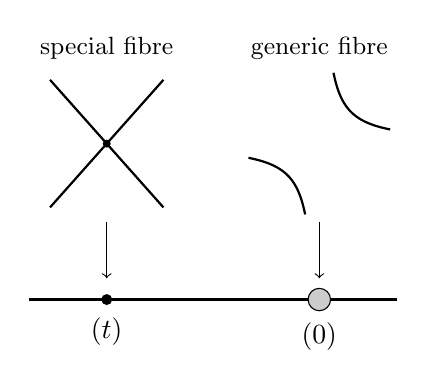
\begin{tikzpicture}[scale=0.9]
% base
\draw[thick] (-2.6,-2.2)--(2.6,-2.2);
\fill (-1.5,-2.2) circle (2.2pt) node[below=3pt]{\((t)\)};
\draw[fill=gray!40] (1.5,-2.2) circle (4.5pt) node[below=5pt]{\((0)\)};
% special fibre: two lines
\draw[thick] (-2.3,-0.9)--(-0.7,0.9) (-2.3,0.9)--(-0.7,-0.9);
\fill (-1.5,0) circle (1.6pt);
\node at (-1.5,1.35) {\small special fibre};
% generic fibre: hyperbola
\draw[thick,domain=0.2:1,samples=40,smooth] plot ({1.5+\x},{0.2/\x});
\draw[thick,domain=-1:-0.2,samples=40,smooth] plot ({1.5+\x},{0.2/\x});
\node at (1.5,1.35) {\small generic fibre};
\draw[->] (-1.5,-1.1)--(-1.5,-1.9);
\draw[->] (1.5,-1.1)--(1.5,-1.9);
\end{tikzpicture}
\end{column}
\begin{column}{0.48\textwidth}
\textbf{The closed point \((t)\).} Here \(t=0\). The fibre is \(\SR(\mathcal M)\): the special fibre.
\par\medskip
\textbf{The generic point \((0)\).} Here \(t\) is invertible. The fibre is the \emph{generic fibre}: a scheme over the field \(\C((t))\).
\par\medskip
\textbf{Formal.} The \(F_i\) are power series in \(t\). They need not converge, so we cannot give \(t\) a numerical value. Part 7 repairs this.
\par\medskip
\textbf{Next time.} Part 5: the construction of \(D_1\). Part 6: the generic fibre is smooth.
\end{column}
\end{columns}
\end{frame}

\partslide{5}{The \(G\)-equivariant first-order deformation of \(\mathcal M\)}{We construct the first-order deformation \(D_1\) that Part 4 starts from, and check that it is flat and \(G\)-equivariant.}

\begin{frame}{What is left: a \(G\)-equivariant first-order deformation}
\textbf{Where we are.} Part 4: every \(G\)-equivariant first-order deformation of \(\SR(\mathcal M)\) extends to a formal family. We have not yet written one down.
\par
\textbf{What we must find.} Sixteen cubics \(H_1,\dots,H_{16}\) such that the equations
\[
\boxed{m_i+t\,H_i=0,\qquad i=1,\dots,16}
\]
\begin{itemize}
\setlength{\itemsep}{1pt}
\item are \emph{flat}: every relation among the \(m_i\) lifts (next slide);
\item are \emph{\(G\)-equivariant}: \(G\) permutes the sixteen equations.
\end{itemize}
\textbf{The plan.}
\begin{enumerate}
\setlength{\itemsep}{1pt}
\item \emph{A building block.} Multiply some of the cubics by one fraction of monomials. For example \(abf\) becomes \(abf+t\,ace\). We check that this is flat.
\item \emph{Symmetrize.} Apply the six symmetries of \(G\) to the building block and add the results. The sum is flat and \(G\)-equivariant.
\item \emph{Ours.} Do this for ten building blocks, and add them with coefficients \(1,\dots,10\).
\end{enumerate}
\end{frame}

\begin{frame}{How to test flatness at first order}
\textbf{Relations.} A relation (or syzygy) among the generators is a row \(r=(r_i)\) of polynomials with \(\sum_i r_im_i=0\). The relations are the kernel of \(d_1\) in the minimal free resolution
\(\ \cdots\to F_2\xrightarrow{d_2}F_1\xrightarrow{d_1}S\to S/I\to0\).
\par
\textbf{Artin's Criterion.} The quotient \(S_B/J\) is flat over \(\mathbb C[t]/(t^2)\)
if every such relation lifts, meaning that we can choose
polynomials \(r'_i\) so that
\[
\sum_i(r_i+t r'_i)(m_i+tH_i)=0.
\]
\textbf{Pair relations.} Take two generators \(m_i,m_j\) and let \(\ell\) be their least common multiple. Then \(\ \frac{\ell}{m_i}\cdot m_i-\frac{\ell}{m_j}\cdot m_j=0\).
For an ideal generated by monomials, the pair relations generate all relations. So it is enough to lift the pair relations.
\src{G. Alecci and M. Graffeo, \emph{Computations in Algebraic Geometry} (Unicamp), Theorem~3.15 \cite{Graffeo-Alessi}.}
\end{frame}

\begin{frame}{Simple maps}
\textbf{What we are looking for.} A choice of corrections \(H=(H_1,\dots,H_{16})\): sixteen cubics, one for each generator \(m_i\). The equations become \(m_i+t\,H_i\).
\par\medskip
\textbf{Definition.} Choose two monomials \(p\) and \(q\) of the same degree, with no common letter. The \emph{simple map} of the fraction \(p/q\) is the choice of corrections
\[
\boxed{H_i=\begin{cases}\dfrac{p}{q}\cdot m_i&\text{if }q\text{ divides }m_i,\\[6pt]0&\text{otherwise.}\end{cases}}
\]
In words: in every generator that contains \(q\), replace the factor \(q\) by \(p\).
\par\medskip
\textbf{A convention.} If a correction \(H_i\) lies in \(I\), we replace it by \(0\). This does not change the ideal generated by the \(m_i+t\,H_i\), because \(t\cdot H_i\) is then a combination of \(t\,m_1,\dots,t\,m_{16}\).
\par\medskip
\textbf{The question.} A simple map is only a choice of corrections. It is a first-order deformation when it is flat: when every relation lifts.
\end{frame}

\begin{frame}{An example: \(abf\) becomes \(abf+t\,ace\)}
\textbf{The simple map of \(ce/bf\).} Two generators contain \(bf\): \(abf\) and \(bdf\).
\[
\frac{ce}{bf}\cdot abf=ace,\qquad\frac{ce}{bf}\cdot bdf=cde\in I.
\]
So \(H_1=ace\), and all the other corrections are \(0\): the cubic \(abf\) becomes \(abf+t\,ace\), and the other fifteen do not change.
\par\medskip
\textbf{Lifting one relation.} Take the pair relation of \(abf\) and \(abg\): \(\ g\cdot abf-f\cdot abg=0\). Here \(r=(g,-f,0)\) on the cubics \(abf,\ abg,\ acg\). With the same \(r\) we do not get \(0\):
\[
g\,({\color{green!55!black}abf}+t\,ace)-f\cdot{\color{green!55!black}abg}=t\,aceg=t\,e\cdot acg.
\]
\underline{The extra term is a multiple of the cubic \(acg\).} So take \(r'=(0,0,-e)\):
\[
\underbrace{g}_{r_1+t\,r_1'}(abf+t\,ace)\ +\ \underbrace{(-f)}_{r_2+t\,r_2'}\,abg\ +\ \underbrace{(0-t\,e)}_{r_3+t\,r_3'}\,acg\ =\ 0.
\]
\end{frame}

\begin{frame}{This simple map is flat}
We must lift every pair relation.
\par\bigskip
\textbf{Pairs without \(abf\).} Neither cubic changes, so there is nothing to do.
\par\bigskip
\textbf{Pairs with \(abf\).} In the example of the last slide, the remainder is \(t\,aceg\). It contains the cubic \(acg\), which did not change when we applied the simple map. So we could cancel it. The same happens for every other pair with \(abf\): the remainder contains a cubic that did not change, namely \(acg\), \(ach\) or \(cde\). So it can be cancelled.
\par\bigskip
\textbf{Conclusion.} Every pair relation lifts, and the pair relations generate all relations. By Artin's criterion,
\[
\boxed{abf+t\,ace,\ \text{the other fifteen unchanged: a flat first-order deformation.}}
\]
\end{frame}

\begin{frame}{From a simple map to a \(G\)-equivariant deformation}
\textbf{Six simple maps.} Apply each \(\gamma\in G\) to the letters of ``\(abf\) becomes \(abf+t\,ace\)'':
\[
\begin{array}{c|cccccc}
\gamma&1&\sigma&\tau&\sigma\tau&\tau\sigma&\sigma\tau\sigma\\\hline
\text{cubic}&abf&adh&cde&efg&cfh&bdg\\
\text{correction}&ace&aeg&abc&agh&bcg&cgh
\end{array}
\]
Each column is a simple map: sixteen corrections, only one of them not zero.
\par
\textbf{The \(G\)-equivariant deformation is their sum.} Blend all the simple maps in the orbit of the first one into one first-order deformation. The sixteen cubics become
\[
\boxed{\begin{array}{c}
abf+t\,ace,\quad adh+t\,aeg,\quad cde+t\,abc,\quad efg+t\,agh,\quad cfh+t\,bcg,\quad bdg+t\,cgh,\\[3pt]
\text{and the other ten unchanged: }abg,\ abh,\ acg,\ ach,\ bdf,\ beg,\ ceg,\ ceh,\ def,\ dfh.
\end{array}}
\]
\textbf{It is flat.} Each column is flat: it is the example with the letters renamed. And a sum of flat choices of \(H\) is flat.
\par
\textbf{It is \(G\)-equivariant.} An element of \(G\) sends each column to another column: it permutes the six deformed cubics. It also moves the other ten cubics among themselves, for example \(\sigma(abg)=ach\). So it sends the list of sixteen to itself.
\end{frame}

\begin{frame}{Our first-order deformation: ten simple maps}
\begin{center}
\small\renewcommand{\arraystretch}{0.85}
\begin{tabular}{ccll}
times&fraction&what it does&images under \(G\)\\\hline
\(1\)&\(ce/bf\)&\(abf\mapsto ace\)&\(6\)\\
\(2\)&\(ce/af\)&\(abf\mapsto bce\)&\(6\)\\
\(3\)&\(c^2e/abf\)&\(abf\mapsto c^2e\)&\(6\)\\
\(4\)&\(ce^2/abf\)&\(abf\mapsto ce^2\)&\(6\)\\
\(5\)&\(ce/ab\)&\(abf\mapsto cef\)&\(6\)\\
\(6\)&\(df/cg\)&\(acg\mapsto adf\)&\(3\)\\
\(7\)&\(d^2f/acg\)&\(acg\mapsto d^2f\)&\(2\)\\
\(8\)&\(fh/ab\)&\(abf\mapsto f^2h,\quad abg\mapsto fgh,\quad abh\mapsto fh^2\)&\(6\)\\
\(9\)&\(ef/ab\)&\(abf\mapsto ef^2,\quad abh\mapsto efh\)&\(6\)\\
\(10\)&\(ac/bf\)&\(abf\mapsto a^2c,\quad bdf\mapsto acd\)&\(6\)
\end{tabular}
\end{center}
Blend each row as on the last slide. Then blend the ten blends into a big one, with the following coefficients (which will be explained later): row 1 once, row 2 twice, \dots, row 10 ten times.
\par
For example \(H_1=ace+2\,bce+3\,c^2e+4\,ce^2+5\,cef+8\,f^2h+9\,ef^2+10\,a^2c\).
\par
This is our \(G\)-equivariant first-order deformation.
\src{\textbf{Catch:} the ten rows come from a computer enumeration of the \(6636\) fractions of degree at most \(3\): up to \(G\) and changes of coordinates, no other is flat. But 10 rows \emph{are} human-checkable.}
\end{frame}

\partslide{6}{The generic fibre is smooth}{By contradiction. A singular point of the generic fibre would specialize to a point of \(\SR(\mathcal M)\). We rule this out on one face: the triangle \(beh\).}

\begin{frame}{A dummy example: how the contradiction works}
Take the family over \(\C[[t]]\) given by one equation:
\[
\boxed{f(x,y,t)=xy-t^2.}
\]
\textbf{Special fibre} (\(t=0\)): \(xy=0\), two lines, singular at the origin.
\par\medskip
\textbf{Generic fibre} (\(t\) invertible): suppose \(P\) is a singular point. On a fixed fibre \(t\) is a constant, so we differentiate only in \(x\) and \(y\):
\[
f_x=y=0,\qquad f_y=x=0.
\]
But \(P\) also satisfies \(f=0\). Substituting \(x=y=0\) gives
\[
\boxed{0=t^2,}
\]
which is impossible when \(t\) is invertible. So the generic fibre is smooth.
\par\medskip
\textbf{For the triangle:} the same three steps, with \(df+t^2p(u,v)+\cdots\) in place of \(xy-t^2\).
\end{frame}

\begin{frame}{A singular point specializes to the special fibre}
\textbf{What we are doing.} This is where the proof that the generic fibre is smooth starts. We argue by contradiction: assume there is a singular point \(P\) on the generic fibre, and specialize it to the special fibre.
\par\bigskip
\textbf{Input.} The family \(\mathcal X\to\operatorname{Spec}\C[[t]]\), and a \emph{hypothetical} singular point \(P\) of its generic fibre.
\par\bigskip
\textbf{Output.} If \(P\) existed: a singular point \(Q\) of the special fibre \(\SR(\mathcal M)\) with \(P\leadsto Q\). So \(Q\) lies on a triangle, an edge or a vertex of \(\mathcal M\).
\par\bigskip
\textbf{Reminder.} \(P\leadsto Q\) means \(Q\in\overline{\{P\}}\): the point \(Q\) is a specialization of \(P\).
\src{Stacks Project, Definition 5.19.1, Tag 0061.}
\end{frame}

\begin{frame}{The manoeuvre}
\textbf{What we are doing.} We describe the same family near \(Q\) with fewer equations and fewer coordinates.
\par\bigskip
\textbf{Input.} The family near \(Q\): sixteen equations \(F_1,\dots,F_{16}\) in seven affine coordinates.
\par\bigskip
\textbf{Two operations.}
\begin{enumerate}
\setlength{\itemsep}{8pt}
\item \emph{Discard.} If some of the sixteen cubics already generate the special fibre near \(Q\), then their deformed versions generate the family near \(Q\). This uses flatness and Nakayama.
\item \emph{Solve.} Some of the remaining equations can be solved for some of the coordinates, by the implicit function theorem. Those coordinates disappear.
\end{enumerate}
\par\bigskip
\textbf{Output.} A few equations in a few coordinates, near \(Q\).
\end{frame}

\begin{frame}{A particular case: \(Q\) on the triangle \(beh\)}
\textbf{The ambient space.} \(\Pj^7\), with eight homogeneous coordinates
\[
[a:b:c:d:e:f:g:h].
\]
\textbf{The special fibre.} \(\SR(\mathcal M)\): the points where the sixteen monomials vanish.
\par\medskip
\textbf{The hypothesis.} \(P\) is a singular point of the generic fibre. We want a contradiction.
\par\medskip
\textbf{Its specialization.} \(P\leadsto Q\), and \(Q\) is a singular point of the special fibre. It can land on any triangle, edge or vertex of \(\mathcal M\).
\par\medskip
\textbf{Now consider the following particular case.} \(Q\) lands on the triangle \(beh\): the coordinates of \(Q\) in the slots \(b,e,h\) are nonzero, and the other five are zero:
\[
\boxed{Q=[\,0:b:0:0:e:0:0:h\,],\qquad b,e,h\ne0.}
\]
The nonzero slots \(\{b,e,h\}\) are a triangle of \(\mathcal M\). The other cases come later.
\end{frame}

\begin{frame}{The triangle \(beh\) in the link of \(b\)}
\begin{columns}[c]
\begin{column}{0.5\textwidth}
\centering
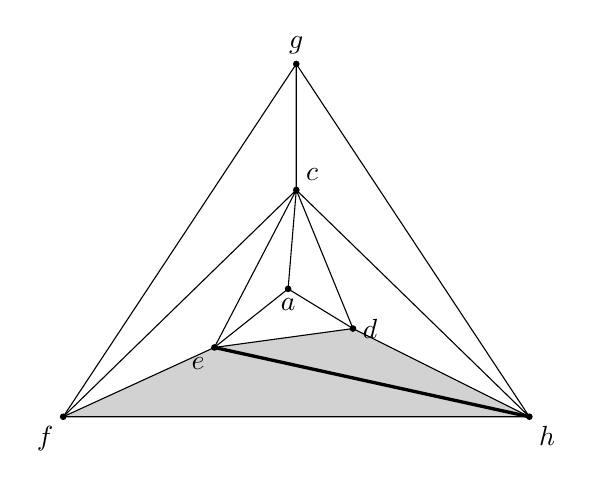
\begin{tikzpicture}[scale=0.8,line join=round]
\coordinate (g) at (0,3.3);
\coordinate (f) at (-3.7,-2.3);
\coordinate (h) at (3.7,-2.3);
\coordinate (c) at (0,1.3);
\coordinate (e) at (-1.3,-1.2);
\coordinate (d) at (0.9,-0.9);
\coordinate (a) at (-0.13,-0.27);
\fill[gray!35] (e)--(f)--(h)--cycle;
\fill[gray!35] (d)--(e)--(h)--cycle;
\draw (f)--(g)--(h)--cycle;
\draw (c)--(f) (c)--(g) (c)--(h) (c)--(e) (c)--(d) (c)--(a);
\draw (e)--(f) (d)--(h) (d)--(e) (a)--(d) (a)--(e);
\draw[very thick] (e)--(h);
\foreach \p/\pos in {g/above,f/below left,h/below right,c/above right,e/below left,d/right,a/below}
  \fill (\p) circle (1.5pt) node[\pos]{\(\p\)};
\end{tikzpicture}
\end{column}
\begin{column}{0.48\textwidth}
\textbf{Remember the link of \(b\)} (Part 2): what we see from the vertex \(b\).
\par\medskip
\textbf{Where our triangle is.} The thick edge \(eh\) is the triangle \(beh\). The two grey triangles \(deh\) and \(efh\) are the two tetrahedra \(bdeh\) and \(befh\) that contain it.
\end{column}
\end{columns}
\end{frame}

\begin{frame}{The triangle \(beh\) inside \(\mathcal M\)}
\begin{columns}[c]
\begin{column}{0.48\textwidth}
\centering
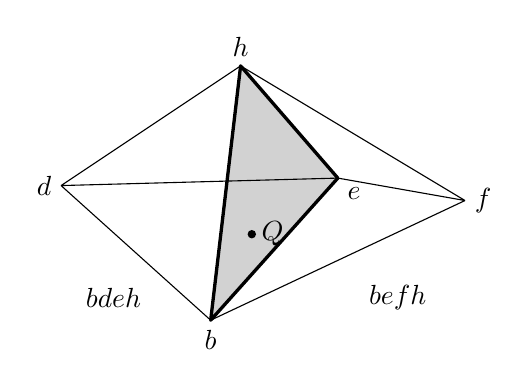
\begin{tikzpicture}[scale=0.95,line join=round]
\coordinate (b) at (-0.6,-1.7);
\coordinate (h) at (-0.2,1.7);
\coordinate (e) at (1.1,0.2);
\coordinate (d) at (-2.6,0.1);
\coordinate (f) at (2.8,-0.1);
\fill[gray!35] (b)--(e)--(h)--cycle;
\draw (d)--(b) (d)--(h) (d)--(e);
\draw (f)--(b) (f)--(h) (f)--(e);
\draw[very thick] (b)--(e)--(h)--cycle;
\fill (-0.05,-0.55) circle (1.6pt) node[right]{\(Q\)};
\node[below] at (b) {\(b\)};
\node[above] at (h) {\(h\)};
\node[below right] at (e) {\(e\)};
\node[left] at (d) {\(d\)};
\node[right] at (f) {\(f\)};
\node at (-1.9,-1.4) {\(bdeh\)};
\node at (1.9,-1.4) {\(befh\)};
\end{tikzpicture}
\par\smallskip
\(Q\) lands in \(beh\)\\[3pt]
\(Q=[\,0:b:0:0:e:0:0:h\,]\)
\end{column}
\begin{column}{0.5\textwidth}
\textbf{In the sphere \(\mathcal M\).} The triangle \(beh\) (grey) is a face of exactly two tetrahedra: \(bdeh\) and \(befh\).
\par\medskip
\textbf{In \(\Pj^7\).}
\begin{itemize}
\setlength{\itemsep}{6pt}
\item each tetrahedron is a \(\Pj^3\);
\item the triangle is the \(\Pj^2\) where they meet.
\end{itemize}
\par\medskip
\textbf{The rule.} A point is drawn in the interior of the face whose vertices are its nonzero slots.
\par\medskip
So a point is in the interior of the edge \(eh\) if \(e,h\ne0\) and all its other slots are zero.
\end{column}
\end{columns}
\src{\textcolor{red}{The explanation of the rule is left for later.}}
\end{frame}

\begin{frame}{The open set \(b,e,h\ne0\)}
\begin{columns}[c]
\begin{column}{0.64\textwidth}
\textbf{Remember.} A point of \(\SR(\mathcal M)\) is in the interior of the edge \(eh\) if \(e,h\ne0\) and all its other coordinates are zero.
\par\smallskip
\textbf{Now let \(b\) be nonzero too.}
\begin{itemize}
\setlength{\itemsep}{2pt}
\item \(b,e,h\ne0\) and all other coordinates zero: the point is in the interior of the triangle \(beh\).
\item \(b,e,h\ne0\) and something else nonzero: the point is in the interior of one of the two tetrahedra that have \(beh\) on their boundary: \(bdeh\) if \(d\ne0\), \(befh\) if \(f\ne0\).
\end{itemize}
\textbf{Nothing else of \(\SR(\mathcal M)\) is in this open set.} The nonzero coordinates of a point form a face, and the only faces containing \(b,e,h\) are \(beh\), \(bdeh\), \(befh\).
\end{column}
\begin{column}{0.34\textwidth}\centering
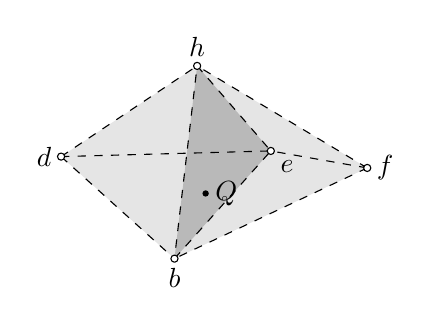
\begin{tikzpicture}[scale=0.72,line join=round]
\coordinate (b) at (-0.6,-1.7);
\coordinate (h) at (-0.2,1.7);
\coordinate (e) at (1.1,0.2);
\coordinate (d) at (-2.6,0.1);
\coordinate (f) at (2.8,-0.1);
\fill[gray!20] (d)--(b)--(e)--(h)--cycle;
\fill[gray!20] (f)--(b)--(e)--(h)--cycle;
\fill[gray!55] (b)--(e)--(h)--cycle;
\draw[dashed] (d)--(b) (d)--(h) (d)--(e) (f)--(b) (f)--(h) (f)--(e) (b)--(e)--(h)--cycle;
\foreach \p/\pos in {b/below,h/above,e/below right,d/left,f/right}
  \draw[fill=white] (\p) circle (1.8pt) node[\pos]{\(\p\)};
\fill (-0.05,-0.55) circle (1.6pt) node[right]{\(Q\)};
\end{tikzpicture}
\par\smallskip
Every point inside the triangle is in the open set, not only \(Q\).
\end{column}
\end{columns}
\end{frame}

\begin{frame}{The equations on the open set}
\textbf{We now work locally.} We replace \(\Pj^7\) by an open set that contains \(Q\): the points with \(b,e,h\ne0\). Being singular at \(Q\) is a local question.
\par\medskip
\textbf{Claim.} On this open set, the sixteen monomials have the same zeros as four equations:
\[
\boxed{a=0,\qquad c=0,\qquad g=0,\qquad df=0.}
\]
\textbf{Step 1: four monomials give the four equations.} Since \(b,e,h\ne0\), we can divide by them:
\[
abh=0\Rightarrow a=0,\qquad ceh=0\Rightarrow c=0,\qquad beg=0\Rightarrow g=0,\qquad bdf=0\Rightarrow df=0.
\]
\textbf{Step 2: the other twelve add nothing.} Each contains \(a\), or \(c\), or \(g\), or both \(d\) and \(f\), so it vanishes once \(a=c=g=0\) and \(df=0\):
\begin{center}
\begin{tabular}{ll@{\qquad}ll}
contains \(a\):&\(abf,\ abg,\ acg,\ ach,\ adh\)&contains \(g\):&\(bdg,\ efg\)\\
contains \(c\):&\(cde,\ ceg,\ cfh\)&contains \(d\) and \(f\):&\(def,\ dfh\)
\end{tabular}
\end{center}
\src{\textcolor{red}{This slide needs verification (not complicated, just need to check).}}
\end{frame}

\begin{frame}{From sixteen equations to four}
Each monomial \(m_i\) has its deformed equation \(F_i=m_i+tH_i+t^2K_i+\cdots\) We work on the open set \(b,e,h\ne0\).
\begin{enumerate}
\setlength{\itemsep}{9pt}
\item \textbf{The monomials} (last slide). The sixteen monomials vanish on the same locus as four of them:
\[
m_3=abh,\qquad m_{12}=ceh,\qquad m_9=beg,\qquad m_7=bdf.
\]
\item \textbf{At \(t=0\).} There \(F_i=m_i\). So the sixteen \(F_i\) vanish on the same locus as \(F_3,\ F_{12},\ F_9,\ F_7\). This is obvious: it is step 1 again.
\item \textbf{For \(t\) invertible.} Do the sixteen \(F_i\) still vanish on the same locus as \(F_3,\ F_{12},\ F_9,\ F_7\)?
\par\smallskip
This is not obvious: the new terms \(tH_i+\cdots\) of the other twelve need not be combinations of the four.
\par\smallskip
\textbf{The answer is yes}, because the family is flat (flatness and Nakayama's lemma).
\end{enumerate}
\src{Step 3 is proved in a formal neighbourhood of each point \(Q\) of the triangle. \textcolor{red}{I will confirm this slide later.}}
\end{frame}

\begin{frame}{From four equations to one}
\textbf{Where we are.} Four equations, \(F_3,\ F_{12},\ F_9,\ F_7\), on the open set \(b,e,h\ne0\).
\par\smallskip
\textbf{Coordinates.} Since \(b\ne0\), we set \(b=1\). We write \(e=u\), \(h=v\), so \(u,v\ne0\). Seven coordinates remain:
\[
a,\ c,\ g,\ d,\ f,\ u,\ v.
\]
\textbf{At \(t=0\).} The four equations are the four monomials. In the old and in the new notation:
\[
\begin{array}{l@{\quad}l@{\qquad\qquad}l@{\quad}l}
F_3:& abh=v\,a & F_9:& beg=u\,g\\[4pt]
F_{12}:& ceh=uv\,c & F_7:& bdf=df
\end{array}
\]
So the equations are
\[
v\,a=0,\qquad uv\,c=0,\qquad u\,g=0,\qquad df=0.
\]
Divide the first three by \(u\) and \(v\): they say \(a=0,\ c=0,\ g=0\).
\par\medskip
What is left is one equation, \(df=0\), in the coordinates \(d,f,u,v\).
\end{frame}

\begin{frame}{Solving for \(a,\ c,\ g\)}
\textbf{Where we are.} Near \(Q\) the family is the zero locus of \(F_3,\ F_{12},\ F_9,\ F_7\), in the coordinates \(a,c,g,d,f,u,v\) and the parameter \(t\).
\par
\textbf{At \(t=0\)} (last slide). Three equations, \(F_3=v\,a=0\), \(F_{12}=uv\,c=0\), \(F_9=u\,g=0\), said
\[
a=0,\qquad c=0,\qquad g=0;
\]
one was left, \(F_7=df=0\).
\par
\textbf{Now with \(t\).} There will be \(A,\ C,\ G\) in \(d,f,u,v,t\) only, zero at \(t=0\), with
\[
\boxed{F_3=F_{12}=F_9=0\quad\Longleftrightarrow\quad a=A,\quad c=C,\quad g=G.}
\]
\textbf{These are two claims.}
\begin{itemize}
\setlength{\itemsep}{0pt}
\item[\(\Rightarrow\)] If the three equations hold, then \(a,c,g\) must be \(A,C,G\).
\item[\(\Leftarrow\)] If we set \(a=A,\ c=C,\ g=G\), then the three equations hold.
\end{itemize}
At \(t=0\) both are clear, since \(u,v\ne0\). With \(t\), both need a proof.
\par
\textbf{What this gives.} A point of the family depends only on \(d,f,u,v,t\).
\end{frame}

\begin{frame}{The one equation left}
\textbf{The fourth equation.}
\[
F_7=bdf+t\,(10\,acd+10\,cfg)+t^2K_7+\cdots
\]
\textbf{Substitute} \(b=1\) and the solutions \(a=A\), \(c=C\), \(g=G\) of the last slide.
\begin{itemize}
\setlength{\itemsep}{0pt}
\item \(bdf\) becomes \(df\).
\item Each term of \(10\,acd+10\,cfg\) contains two of \(a,c,g\). Each of \(A,C,G\) is zero at \(t=0\), so it is divisible by \(t\). So \(t\,(10\,acd+10\,cfg)\) becomes divisible by \(t^3\): no \(t\) term is left.
\end{itemize}
\textbf{The result.} Near \(Q\) the family is given by one equation in \(d,f,u,v\) and \(t\):
\[
\boxed{\Phi(d,f,u,v,t)=df+t^2B(d,f,u,v)+t^3(\cdots)=0,}
\]
and at \(d=f=0\) the coefficient \(B\) is \(\ B(0,0,u,v)=p(u,v)=-8u^2-20uv-8v^2-20u-20v-8\).
\par
Compare the dummy example \(xy-t^2\): the same shape.
\src{\textcolor{red}{\(H_7\) and \(p\) are copied, not re-derived.}}
\end{frame}

\begin{frame}{What a singular point near the triangle would satisfy}
\textbf{The hypothesis.} \(P\) is a singular point of the generic fibre, and \(P\leadsto Q\) in the triangle. As in the dummy example, at \(P\):
\[
\Phi=0,\qquad \Phi_d=\Phi_f=\Phi_u=\Phi_v=0 .
\]
\textbf{Step 1: \(d\) and \(f\) are small.} Since \(\Phi=df+t^2B+\cdots\),
\[
\Phi_d=f+t^2(\cdots)=0,\qquad \Phi_f=d+t^2(\cdots)=0 .
\]
So at \(P\) both \(d\) and \(f\) are divisible by \(t^2\).
\par
\textbf{Step 2: substitute.} Then \(df\) is divisible by \(t^4\), and \(B(d,f,u,v)=p(u,v)+t^2(\cdots)\). The equations \(\Phi=0\), \(\Phi_u=0\), \(\Phi_v=0\) become
\[
t^2p+t^3(\cdots)=0,\qquad t^2p_u+t^3(\cdots)=0,\qquad t^2p_v+t^3(\cdots)=0 .
\]
\textbf{Step 3: divide by \(t^2\) and specialize \(P\leadsto Q\).} The coordinates \((u,v)\) of \(Q\) satisfy
\[
\boxed{p(u,v)=0,\qquad p_u(u,v)=0,\qquad p_v(u,v)=0.}
\]
\src{The full proof makes these steps over a discrete valuation ring; here they are only sketched.}
\end{frame}

\begin{frame}{No singular point near the triangle}
\textbf{Where we are.} A singular point \(P\leadsto Q\) would give a common zero \((u,v)\) of \(p,\ p_u,\ p_v\), where
\[
p=-8u^2-20uv-8v^2-20u-20v-8 .
\]
\textbf{There is none.} The derivatives are
\[
p_u=-16u-20v-20,\qquad p_v=-20u-16v-20 .
\]
\(p_u=p_v=0\) forces \(u=v=-\tfrac59\). There
\[
p\bigl(-\tfrac59,-\tfrac59\bigr)=\tfrac{28}9\ne0 .
\]
\textbf{The same in one line.}
\[
\boxed{p-\tfrac12\bigl(u+\tfrac59\bigr)p_u-\tfrac12\bigl(v+\tfrac59\bigr)p_v=\tfrac{28}{9}.}
\]
\textbf{Conclusion.} No singular point of the generic fibre specializes to the triangle \(beh\).
\end{frame}

\begin{frame}{The other cases}
The same scheme applies to every face of \(\mathcal M\).
\begin{itemize}
\setlength{\itemsep}{12pt}
\item \textbf{Edges.} The edge \(be\) has two ranges of valuations and an exceptional cancellation: \(H_7=10acd+10cfg\).
\item \textbf{Other triangles and edges.} Tables and short calculations.
\item \textbf{Vertices.} Three orbits: \(a\), \(b\), \(d\). The family is \(G\)-equivariant, so \(G\) acts on \(\mathcal X\), and \(\pi\colon\mathcal X\to B\) is \(G\)-equivariant, with \(G\) acting trivially on \(B\): each \(\gamma\) sends every fibre to itself. So one vertex in each orbit is enough.
\end{itemize}
\end{frame}

\partslide{7}{Algebraization}{The formal family over \(\C[[t]]\) is replaced by a family over an algebraic curve.}

\begin{frame}{From a formal family to a family over a curve}
\textbf{Input.} A flat family over \(\C[[t]]\): special fibre \(X\), smooth generic fibre (Parts 4 to 6).
\par
\textbf{Output.} A curve \(C\ni0\) and a flat family in \(\Pj^7\times C\): fibre \(X\) over \(0\), smooth fibres elsewhere.
\begin{columns}[c]
\begin{column}{0.63\textwidth}
\begin{enumerate}
\setlength{\itemsep}{2pt}
\item \emph{Hilbert scheme \(\mathcal H\).} Its points: the subschemes of \(\Pj^7\) with the Hilbert polynomial of \(X\). One of them is \(x=X\).
\item \emph{The formal family is an arc} \(\operatorname{Spec}\C[[t]]\to\mathcal H\): closed point to \(x\), generic point to a point \(\eta\).
\item \emph{Smooth subschemes form an open set} of \(\mathcal H\). It contains \(\eta\) and not \(x\).
\item \emph{\(W\): the closure of \(\eta\).} A variety through \(x\); most of its points are smooth subschemes.
\item \emph{Choose a curve} in \(W\) through \(x\), not inside the bad set.
\end{enumerate}
\end{column}
\begin{column}{0.32\textwidth}\centering
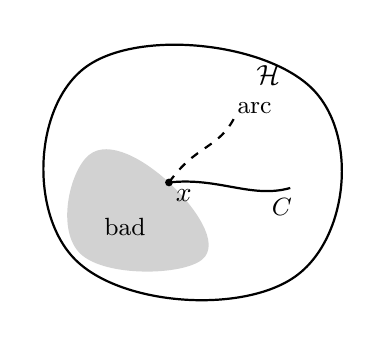
\begin{tikzpicture}[scale=0.7]
\draw[thick] plot[smooth cycle,tension=0.8] coordinates {(-2,-1.6) (2,-1.9) (2.3,1.5) (-1.8,1.9)};
\fill[gray!35] plot[smooth cycle,tension=0.8] coordinates {(-1.9,-1.5) (0.3,-1.6) (-0.3,-0.2) (-1.75,0.3)};
\node at (-1.1,-1.0) {\small bad};
\fill (-0.3,-0.2) circle (2pt) node[below right=-1pt]{\(x\)};
\draw[dashed,thick] (-0.3,-0.2) .. controls (0.2,0.5) and (0.6,0.4) .. (0.9,1.0);
\node at (1.25,1.15) {\small arc};
\draw[thick] (-0.3,-0.2) .. controls (0.6,-0.1) and (1.2,-0.5) .. (1.9,-0.3);
\node at (1.75,-0.65) {\small \(C\)};
\node at (1.5,1.75) {\(\mathcal H\)};
\end{tikzpicture}
\par
{\small Grey: not smooth. Dashed: the formal arc. Solid: the curve chosen.}
\end{column}
\end{columns}
\src{The curve need not be the arc we started with; no convergence of the series is used.}
\end{frame}

\partslide{8}{Conclusion}{What we did, and what is open.}

\begin{frame}{What we did}
\textbf{Theorem (proposed).} \(\SR(\mathcal M)\) has a smoothing, whose smooth fibres are Calabi--Yau threefolds of degree \(20\) in \(\Pj^7\).
\par\medskip
{\small\renewcommand{\arraystretch}{1.15}
\begin{tabular}{>{\raggedright\arraybackslash}p{0.24\textwidth}>{\raggedright\arraybackslash}p{0.36\textwidth}>{\raggedright\arraybackslash}p{0.3\textwidth}}
\textbf{Step}&\textbf{Idea}&\textbf{In this talk}\\ \hline
1. A formal family&an obstruction fixed by \(G\) is zero&argument shown; the computation of \(T^2\) not shown\\
2. Its generic fibre is smooth&a singular point would specialize to a face; there the family is \(df+t^2p+\cdots\)&the triangle \(beh\); the other faces not shown\\
3. Algebraization&a curve in the Hilbert scheme&sketched\\
4. Calabi--Yau&semicontinuity and Riemann--Roch&shown, for every \(3\)-sphere
\end{tabular}}
\par\medskip
\textbf{Around it.} \(\mathcal M\) is one of \(39\) spheres with \(8\) vertices; the known Calabi--Yau threefolds in \(\Pj^7\) are eleven families. Which family the smoothing of \(\mathcal M\) belongs to is not known.
\src{\textbf{Status.} The proof was assembled with AI help and checked by an AI audit. I am verifying it by hand; this is not finished.}
\end{frame}

\begin{frame}{Open questions}
\begin{itemize}
\setlength{\itemsep}{12pt}
\item Is the smoothing the Gulliksen--Negård threefold? A comparison with a del Pezzo construction suggested by Grzegorz is unresolved.
\item Hodge numbers, fundamental group.
\item Other non-polytopal spheres.
\item Human verification of the proof.
\end{itemize}
\par\bigskip
\textbf{Questions for you.}
\begin{enumerate}
\item Which step would you check first?
\item Is there a conceptual reason why this complex smooths?
\end{enumerate}
\end{frame}

%% Frames taken out of v2 (kept, not shown).
\iffalse
% Taken out 26 Nov: the proof of the degree count, replaced by one simple slide in Part 3.
\begin{frame}{\(X\) is a union of copies of \(\Pj^3\), one for each tetrahedron}
\textbf{The pieces.} For a tetrahedron \(F\) of \(\Delta\), let \(\Pj^3_F\subset\Pj^{n-1}\) be the subspace where the coordinates \(x_i\) with \(i\notin F\) are zero. Then \(X=\bigcup_F\Pj^3_F\).
\par\medskip
\textbf{Example.} In \(\mathcal M\) take \(F=abcd\). The vertices not in \(F\) are \(e,f,g,h\).
\begin{itemize}
\setlength{\itemsep}{2pt}
\item Each of \(e=0\), \(f=0\), \(g=0\), \(h=0\) is a hyperplane of \(\Pj^7\).
\item The points on all four hyperplanes form \(\Pj^3_{abcd}\). It is a \(\Pj^3\), with coordinates \(a,b,c,d\).
\item It lies in \(X\). None of the sixteen triples is inside \(abcd\). So each of the sixteen cubics has a factor \(e\), \(f\), \(g\) or \(h\), and is zero there.
\end{itemize}
\par\medskip
\textbf{Why, in general.} Take a point and let \(S\) be the set of its nonzero coordinates. A monomial \(x_N\) is nonzero at the point exactly when \(N\subset S\). So the point is in \(X\) exactly when \(S\) contains no non-face, that is, when \(S\) is a face. Every face of a sphere lies in a tetrahedron \(F\), and \(S\subset F\) says that the point is in \(\Pj^3_F\).
\par\medskip
\textbf{No multiplicities.} The generators \(x_N\) have no squares, so \(I_\Delta\) is radical.
\end{frame}

\begin{frame}{The degree of \(X\) is the number of tetrahedra: proof}
\textbf{Counting points.} The degree of \(X\) is the number of points where a general linear subspace \(L\) of codimension \(3\) meets \(X\).
\begin{itemize}
\setlength{\itemsep}{2pt}
\item \(L\) meets each \(\Pj^3_F\) in one point.
\item Two different \(\Pj^3_F\) meet in a linear subspace of dimension at most \(2\), and \(L\) misses it. So these points are different.
\end{itemize}
One point for each tetrahedron. For \(\mathcal M\): degree \(20\).
\par\medskip
\textbf{The smooth fibre.} The degree is the same for all fibres of a flat family: \(\deg Y=\deg X\).
\end{frame}

% Old Part 3 slides on the canonical bundle (forms with poles; the count on a smooth fibre). Replaced 25 Nov 2026.
\begin{frame}{Forms on a line}
\textbf{Two charts.} \(\Pj^1=\C\cup\{\infty\}\), with coordinate \(x\) on \(\C\) and \(w=1/x\) near \(\infty\).
\par\medskip
\textbf{The form \(dx\).} On \(\C\) it has no zeros and no poles. Near \(\infty\): \(x=1/w\), so \(dx=-\dfrac{dw}{w^{2}}\). A pole of order \(2\) at \(\infty\).
\par\medskip
\textbf{Any form with no pole on \(\C\).} It is \(p(x)\,dx\) with \(p\) a polynomial. At \(\infty\) it is \(-p(1/w)\,w^{-2}\,dw\), and \(p(1/w)\) has a pole or is constant, so the pole at \(\infty\) has order at least \(2\) unless \(p=0\).
\par\medskip
\textbf{Result.} \(\Pj^1\) has no nonzero form without poles. Every nonzero form has \(\ge 2\) poles, counted with order.
\par\medskip
\textbf{The best one.} \(\dfrac{dx}{x}\): simple pole at \(0\), and at \(\infty\) it is \(\dfrac{-dw/w^{2}}{1/w}=-\dfrac{dw}{w}\), a simple pole. No zeros. Residues \(+1\) at \(0\) and \(-1\) at \(\infty\).
\end{frame}

\begin{frame}{Three lines in the plane}
\textbf{What we want.} The canonical bundle is trivial when there is a volume form with no zeros and no poles.
\begin{columns}[c]
\begin{column}{0.36\textwidth}\centering
\begin{tikzpicture}[scale=1.0,line join=round]
\coordinate (A) at (90:1.5); \coordinate (B) at (210:1.5); \coordinate (C) at (330:1.5);
\foreach \a/\b in {A/B,B/C,C/A}
  \draw[thick,shorten <=-0.7cm,shorten >=-0.7cm] (\a)--(\b);
\foreach \p in {A,B,C} \fill (\p) circle (2pt);
\node at ($(A)!0.2!(B)+(-0.28,0.1)$) {\small\(+\)};
\node at ($(A)!0.8!(B)+(-0.28,0.1)$) {\small\(-\)};
\node at ($(B)!0.2!(C)+(0,-0.28)$) {\small\(+\)};
\node at ($(B)!0.8!(C)+(0,-0.28)$) {\small\(-\)};
\node at ($(C)!0.2!(A)+(0.28,0.1)$) {\small\(+\)};
\node at ($(C)!0.8!(A)+(0.28,0.1)$) {\small\(-\)};
\end{tikzpicture}
\par\smallskip
{\small The triangle: three lines in \(\Pj^2\), \(xyz=0\). The signs are the residues.}
\end{column}
\begin{column}{0.62\textwidth}
\textbf{One line.} The best form on \(\Pj^1\) is \(\dfrac{dx}{x}\): no zeros, and two simple poles, at \(0\) and at \(\infty\), with residues \(+1\) and \(-1\).
\par\smallskip
\textbf{Where the poles are.} Exactly at the two points where the line meets its neighbours.
\par\smallskip
\textbf{Gluing.} At each corner two lines meet, one with residue \(+1\) and the other with \(-1\). The two poles cancel: the form passes through the corner.
\par\smallskip
\textbf{Result.} The three lines together carry a form with no zeros and no poles. Their smoothing is a smooth cubic curve, and it has one too: \(K\) is trivial.
\end{column}
\end{columns}
\src{\textcolor{red}{The rule that opposite residues glue is standard (the dualizing sheaf of a nodal curve); I did not check a source.}}
\end{frame}

\begin{frame}{The same for a \(3\)-sphere}
\begin{columns}[c]
\begin{column}{0.36\textwidth}\centering
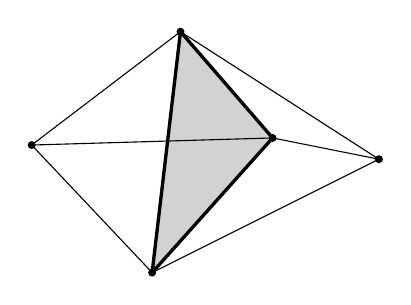
\begin{tikzpicture}[scale=0.9,line join=round]
\coordinate (b) at (-0.6,-1.7);
\coordinate (h) at (-0.2,1.7);
\coordinate (e) at (1.1,0.2);
\coordinate (d) at (-2.3,0.1);
\coordinate (f) at (2.6,-0.1);
\fill[gray!35] (b)--(e)--(h)--cycle;
\draw (d)--(b) (d)--(h) (d)--(e);
\draw (f)--(b) (f)--(h) (f)--(e);
\draw[very thick] (b)--(e)--(h)--cycle;
\foreach \p in {b,h,e,d,f} \fill (\p) circle (1.6pt);
\end{tikzpicture}
\par\smallskip
{\small Two tetrahedra and their common triangle: two \(\Pj^3\)'s meeting along a plane.}
\end{column}
\begin{column}{0.62\textwidth}
\textbf{One \(\Pj^3\).} Every \(3\)-form has poles. The best one is
\[
\frac{dx}{x}\wedge\frac{dy}{y}\wedge\frac{dz}{z}:
\]
no zeros, and simple poles along \(4\) planes. This is what \(K_{\Pj^3}=-4\) planes means.
\par\smallskip
\textbf{Where the poles are.} Exactly on the \(4\) faces of the tetrahedron: the planes where this \(\Pj^3\) meets its neighbours.
\par\smallskip
\textbf{Gluing.} In a sphere every triangle is in exactly two tetrahedra. So every pole is matched by the opposite pole next door, and none is left over.
\par\smallskip
\textbf{Result.} The glued space carries a volume form with no zeros and no poles. A smoothing inherits it.
\end{column}
\end{columns}
\src{This is the picture, not the proof: the proof is on the next two slides. \textcolor{red}{That the signs can be chosen consistently uses that the sphere is orientable; standard, source not checked.}}
\end{frame}

\begin{frame}{Two facts about the glued space}
\textbf{Notation.} A triangulated \(3\)-sphere with \(n\) vertices, \(e\) edges, \(T\) tetrahedra. Its scheme \(X\subset\Pj^{n-1}\).
\par
\textbf{Fact 1: cohomology.} \(H^i(X,\cO_X)\) is the cohomology of the sphere:
\[
\boxed{H^0=\C,\qquad H^1=0,\qquad H^2=0,\qquad H^3=\C.}
\]
\textbf{Fact 2: Hilbert polynomial.} There is no \(m^2\) term and no constant term:
\[
\boxed{\chi(\cO_X(m))=\frac T6\,m^3+\Bigl(e-\frac{7T}6\Bigr)m.}
\]
\textbf{Why Fact 2.} Count the monomials of degree \(m\) by the face they live on:
\[
n+e\,(m-1)+2T\tbinom{m-1}2+T\tbinom{m-1}3 .
\]
A sphere has \(2T\) triangles, and \(n-e+2T-T=0\). Expand.
\par
\textbf{For \(\mathcal M\).} \(n=8\), \(e=28\), \(T=20\): \(\ \chi(\cO_X(m))=\tfrac{10}3m^3+\tfrac{14}3m\).
\src{Fact 2 in general: computed for this talk. \textcolor{red}{Fact 1 in general is standard, but I did not check a source.}}
\end{frame}

\begin{frame}{Why a smooth fibre is Calabi--Yau}
The proof does not glue forms. It counts, on a smooth fibre \(Y\) close to \(X\). \(H\): a hyperplane.
\begin{enumerate}
\setlength{\itemsep}{0pt}
\item \emph{Semicontinuity.} By Fact 1, \(H^1(\cO_Y)=H^2(\cO_Y)=0\) and \(Y\) is connected.
\item \emph{Flatness.} \(Y\) has the Hilbert polynomial of \(X\). So \(\chi(\cO_Y)=0\), and \(h^3(\cO_Y)=1\).
\item \emph{Serre duality.} \(h^0(K_Y)=h^3(\cO_Y)=1\): there is a nonzero section \(s\) of \(K_Y\).
\item \emph{Riemann--Roch.} The \(m^2\) coefficient of \(\chi(\cO_Y(m))\) is \(-\tfrac14K_Y\cdot H^2\). By Fact 2 it is \(0\).
\item \emph{No zeros.} If \(s\) had zeros, they would form a surface \(D\) with \(D\cdot H^2>0\). But \(D\cdot H^2=K_Y\cdot H^2=0\). So \(s\) has no zeros: \(K_Y\simeq\cO_Y\).
\end{enumerate}
\textbf{Result.} The \(m^3\) and \(m\) coefficients are \(\tfrac16H^3\) and \(\tfrac1{12}c_2\cdot H\). So
\[\setlength{\fboxsep}{2pt}
\boxed{K_Y\simeq\cO_Y,\qquad H^1(\cO_Y)=H^2(\cO_Y)=0,\qquad H^3=T,\qquad c_2\cdot H=12e-14T.}
\]
\textbf{Examples.} \(5\)-cell: \(5\) and \(50\), the quintic. \(16\)-cell: \(16\) and \(64\), four quadrics. \(\mathcal M\): \(20\) and \(56\).
\src{The formulas in \(e\), \(T\) and the two checks: computed for this talk.}
\end{frame}

\begin{frame}{The same statement in lower dimensions}
\begin{columns}[t]
\begin{column}{0.31\textwidth}\centering
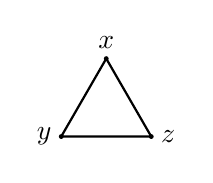
\begin{tikzpicture}[scale=0.55,line join=round]
\coordinate (A) at (90:1.2); \coordinate (B) at (210:1.2); \coordinate (C) at (330:1.2);
\draw[thick] (A)--(B)--(C)--cycle;
\foreach \p/\pos/\n in {A/above/x,B/left/y,C/right/z} \fill (\p) circle (1.6pt) node[\pos]{\(\n\)};
\end{tikzpicture}
\par\smallskip
\textbf{Triangle}\\ (a circle).\\ Three lines in \(\Pj^2\):\\ \(xyz=0\).\\ A limit of smooth cubic curves.
\end{column}
\begin{column}{0.31\textwidth}\centering
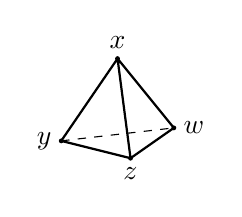
\begin{tikzpicture}[scale=0.55,line join=round]
\coordinate (A) at (0,1.3); \coordinate (B) at (-1.3,-0.6); \coordinate (C) at (0.3,-1.0); \coordinate (D) at (1.3,-0.3);
\draw[dashed] (B)--(D);
\draw[thick] (A)--(B)--(C)--(D)--cycle (A)--(C);
\foreach \p/\pos/\n in {A/above/x,B/left/y,C/below/z,D/right/w} \fill (\p) circle (1.6pt) node[\pos]{\(\n\)};
\end{tikzpicture}
\par\smallskip
\textbf{Tetrahedron}\\ (a \(2\)-sphere).\\ Four planes in \(\Pj^3\):\\ \(xyzw=0\).\\ A limit of smooth quartics: K3 surfaces.
\end{column}
\begin{column}{0.34\textwidth}\centering
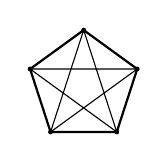
\begin{tikzpicture}[scale=0.55,line join=round]
\foreach \i in {0,...,4} \coordinate (p\i) at ({90+72*\i}:1.3);
\draw[thick] (p0)--(p1)--(p2)--(p3)--(p4)--cycle;
\draw (p0)--(p2)--(p4)--(p1)--(p3)--cycle;
\foreach \i in {0,...,4} \fill (p\i) circle (1.6pt);
\end{tikzpicture}
\par\smallskip
\textbf{\(5\)-cell}\\ (a \(3\)-sphere).\\ Five \(\Pj^3\)'s in \(\Pj^4\):\\ \(x_0x_1x_2x_3x_4=0\).\\ A limit of smooth quintic threefolds.
\end{column}
\end{columns}
\par\smallskip
\textbf{The rule.} One coordinate for each vertex. One equation for each set of vertices that is not a face: the product of its coordinates.
\par
\textbf{Why \(\mathcal M\) is harder.} Above there is one equation, and \(xyzw+t\,q\), with \(q\) a general quartic, is a smoothing. For \(\mathcal M\) there are sixteen equations, to be deformed together.
\end{frame}

\begin{frame}{Provisional: the six missing edges, drawn}
\begin{columns}[c]
\begin{column}{0.5\textwidth}\centering
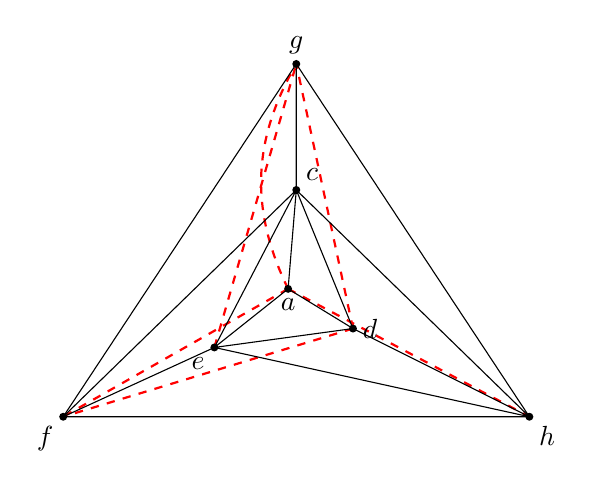
\begin{tikzpicture}[scale=0.8,line join=round]
\coordinate (g) at (0,3.3);
\coordinate (f) at (-3.7,-2.3);
\coordinate (h) at (3.7,-2.3);
\coordinate (c) at (0,1.3);
\coordinate (e) at (-1.3,-1.2);
\coordinate (d) at (0.9,-0.9);
\coordinate (a) at (-0.13,-0.27);
\draw[red,dashed,thick] (a)--(f) (a) to[bend left=28] (g) (a)--(h) (d)--(f) (d)--(g) (e)--(g);
\draw (f)--(g)--(h)--cycle;
\draw (c)--(f) (c)--(g) (c)--(h) (c)--(e) (c)--(d) (c)--(a);
\draw (e)--(f) (d)--(h) (d)--(e) (a)--(d) (a)--(e) (e)--(h);
\foreach \p/\pos in {g/above,f/below left,h/below right,c/above right,e/below left,d/right,a/below}
  \fill (\p) circle (1.8pt) node[\pos]{\(\p\)};
\end{tikzpicture}
\end{column}
\begin{column}{0.48\textwidth}
\textbf{Dashed.} The \(6\) edges not touching \(b\):\\ \(af,\ ag,\ ah,\ df,\ dg,\ eg\).
\par\medskip
They are inside the ball. Drawn flat, they cross the other edges.
\par\medskip
Now every pair of the \(7\) points is joined: \(15+6=21\).
\par\medskip
The \(10\) missing tetrahedra are made of these lines. For example, \(afgh\) is the big triangle \(fgh\) with \(a\) inside: it covers the whole picture.
\par\medskip
The lines do not show which \(10\) of the \(35\) quadruples are the tetrahedra. For that: the 3D model.
\end{column}
\end{columns}
\end{frame}

\begin{frame}{Why the link of \(b\) is a \(2\)-sphere}
A sphere drawn flat: remove one face, flatten the rest. The removed face becomes the outside region. It is like stereographic projection from a point inside that face.
\par\medskip
\begin{columns}[c]
\begin{column}{0.3\textwidth}\centering
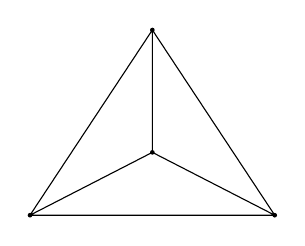
\begin{tikzpicture}[scale=0.42,line join=round]
\coordinate (A) at (0,3.3); \coordinate (B) at (-3.7,-2.3); \coordinate (C) at (3.7,-2.3); \coordinate (O) at (0,-0.4);
\draw (A)--(B)--(C)--cycle (O)--(A) (O)--(B) (O)--(C);
\foreach \p in {A,B,C,O} \fill (\p) circle (2pt);
\end{tikzpicture}
\par\smallskip
\textbf{Tetrahedron.}\\ 3 triangles drawn\\ + the outside \(=4\).
\end{column}
\begin{column}{0.3\textwidth}\centering
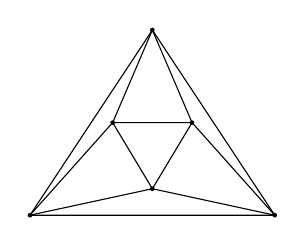
\begin{tikzpicture}[scale=0.42,line join=round]
\coordinate (A) at (0,3.3); \coordinate (B) at (-3.7,-2.3); \coordinate (C) at (3.7,-2.3);
\coordinate (a) at (0,-1.5); \coordinate (b) at (1.2,0.5); \coordinate (c) at (-1.2,0.5);
\draw (A)--(B)--(C)--cycle (a)--(b)--(c)--cycle;
\draw (A)--(b) (A)--(c) (B)--(c) (B)--(a) (C)--(a) (C)--(b);
\foreach \p in {A,B,C,a,b,c} \fill (\p) circle (2pt);
\end{tikzpicture}
\par\smallskip
\textbf{Octahedron.}\\ 7 triangles drawn\\ + the outside \(=8\).
\end{column}
\begin{column}{0.36\textwidth}\centering
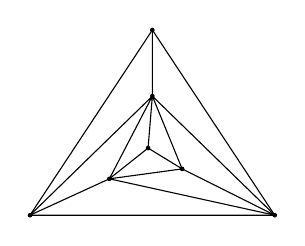
\begin{tikzpicture}[scale=0.42,line join=round]
\coordinate (g) at (0,3.3);
\coordinate (f) at (-3.7,-2.3);
\coordinate (h) at (3.7,-2.3);
\coordinate (c) at (0,1.3);
\coordinate (e) at (-1.3,-1.2);
\coordinate (d) at (0.9,-0.9);
\coordinate (a) at (-0.13,-0.27);
\draw (f)--(g)--(h)--cycle;
\draw (c)--(f) (c)--(g) (c)--(h) (c)--(e) (c)--(d) (c)--(a);
\draw (e)--(f) (d)--(h) (d)--(e) (a)--(d) (a)--(e) (e)--(h);
\foreach \p in {g,f,h,c,e,d,a} \fill (\p) circle (2pt);
\end{tikzpicture}
\par\smallskip
\textbf{Link of \(b\).}\\ 9 triangles drawn\\ + the outside \(fgh\) \(=10\).
\end{column}
\end{columns}
\end{frame}
\begin{frame}{The link of \(b\): what it shows and what it misses}
\begin{columns}[c]
\begin{column}{0.62\textwidth}\centering
\linkofb{1.05}
\end{column}
\begin{column}{0.36\textwidth}
\textbf{It shows.} An edge \(xy\): the triangle \(bxy\). A triangle \(xyz\): the tetrahedron \(bxyz\).
\par\bigskip
\textbf{It misses} what does not touch \(b\):
\begin{itemize}
\setlength{\itemsep}{4pt}
\item \(10\) of the \(20\) tetrahedra;
\item \(6\) of the \(28\) edges:\\ \(af,\ ag,\ ah,\ df,\ dg,\ eg\);
\item \(15\) of the \(40\) triangles.
\end{itemize}
\par\bigskip
The picture is the surface of a ball. The missing tetrahedra fill the inside.
\end{column}
\end{columns}
\end{frame}

\begin{frame}{\(2\)-spheres seen from a vertex}
\begin{columns}[c]
\begin{column}{0.56\textwidth}
\textbf{The model.} Left: the sphere with the vertex \(v\) removed, drawn flat. Right: the solid, to turn by hand.
\par\medskip
\textbf{Regular.} Tetrahedron, cube, octahedron, dodecahedron, icosahedron.
\par\medskip
\textbf{Other \(2\)-spheres.} Double pyramids with \(5\) and \(7\) vertices. The link of \(b\) in \(\mathcal M\). The links of \(7\) and of \(1\) in Barnette's sphere.
\par\medskip
\textbf{Seen from.} Any vertex: use the arrows.
\end{column}
\begin{column}{0.42\textwidth}\centering
\linkofb{0.5}
\par
{\small One of them: the link of \(b\) in \(\mathcal M\).}
\end{column}
\end{columns}
\src{In the live version this slide is the model itself, with all its buttons.}
\end{frame}

\begin{frame}{\(3\)-spheres seen from a vertex}
\textbf{The model.} A \(3\)-sphere with the vertex \(v\) removed, drawn in space. The link of \(v\) is a surface. The cells that do not touch \(v\) fill its inside. The cells at \(v\) are outside.
\par\medskip
\textbf{Regular.} \(5\)-cell, \(16\)-cell, \(600\)-cell, tesseract, \(24\)-cell, \(120\)-cell.
\par\medskip
\textbf{Other \(3\)-spheres.} Double pyramids with \(6\) and \(7\) vertices. Cyclic polytopes with \(7\) and \(8\) vertices. \(\mathcal M\). Barnette's sphere.
\par\medskip
\textbf{Seen from.} Any vertex: use the arrows. The tetrahedra can be shown one by one.
\src{In the live version this slide is the model itself, with all its buttons.}
\end{frame}
\begin{frame}{Why the glued space looks like a Calabi--Yau threefold}
\begin{columns}[c]
\begin{column}{0.64\textwidth}
\textbf{The space.} \(X\): one \(\Pj^3\) for each tetrahedron of a triangulated \(3\)-sphere, glued as the tetrahedra are.
\par\medskip
\textbf{Canonical class.} On \(\Pj^3\), \(K=-4\) planes. Each \(\Pj^3\) is glued to its neighbours along exactly \(4\) planes: the \(4\) faces of its tetrahedron. The two cancel.
\par\medskip
\textbf{One dimension down.} One \(\Pj^2\) for each triangle of a \(2\)-sphere. On \(\Pj^2\), \(K=-3\) lines, and a triangle has \(3\) sides. The tetrahedron gives \(xyzw=0\), which deforms to smooth quartics: K3 surfaces.
\par\medskip
\textbf{This is not a proof.} \(X\) is not smooth. The proof is on the next two slides: it looks at a smooth fibre \(Y\) near \(X\).
\end{column}
\begin{column}{0.34\textwidth}\centering
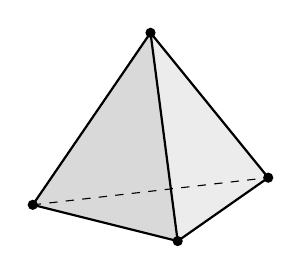
\begin{tikzpicture}[scale=1.15,line join=round]
\coordinate (A) at (0,1.3); \coordinate (B) at (-1.3,-0.6); \coordinate (C) at (0.3,-1.0); \coordinate (D) at (1.3,-0.3);
\fill[gray!30] (A)--(B)--(C)--cycle;
\fill[gray!15] (A)--(C)--(D)--cycle;
\draw[dashed] (B)--(D);
\draw[thick] (A)--(B)--(C)--(D)--cycle (A)--(C);
\foreach \p in {A,B,C,D} \fill (\p) circle (1.6pt);
\end{tikzpicture}
\par\smallskip
{\small One tetrahedron: a \(\Pj^3\). Its \(4\) faces: the \(4\) planes where it meets its neighbours.}
\end{column}
\end{columns}
\end{frame}
\fi

\begin{frame}{\(T^2\) is a sum of \(27\) lines}
\textbf{\(G\) acts on \(T^2\)}, because it permutes the variables. So \(T^2\) is a representation of \(G\). Does it contain the trivial representation?
\par
\textbf{The lines.} \(T^2\) is a direct sum of \(27\) lines. Each line has a label, a fraction of monomials. \(G\) permutes the lines: there are nine orbits, of three lines each. One label from each orbit:
\[
\frac{a^2}{cg},\ \ \frac{a^2}{df},\ \ \frac{a^3}{def},\ \ \frac{b^2}{df},\ \ \frac{b^2}{eh},\ \ \frac{b^3}{ceh},\ \ \frac{ae}{bh},\ \ \frac{ae}{cg},\ \ \frac{ae}{df}.
\]
\textbf{One line.} Take \(a^2/(cg)\). In the link of \(a\), the vertices \(c\) and \(g\) single out two regions: one around \(b\) and \(de\), one around \(ef\) and \(h\). The line is
\[
\C^2/\,\C\,(1,1),
\]
with one coordinate for each region.
\par
\textbf{The other lines} are the same: two regions, in the link of a vertex or of an edge.
\src{The lines and the regions: \cite{AC}, Proposition 11 and Theorem 13. \textcolor{red}{Not re-checked for this slide.}}
\end{frame}

\begin{frame}{Each line of \(T^2\) is flipped}
\textbf{One line.} \(\sigma=(b\ h)(c\ g)(d\ f)\) fixes the label \(a^2/(cg)\), and exchanges its two regions. So on the line \(\C^2/\,\C\,(1,1)\) it acts by \(\sigma(u,v)=(v,u)\). But
\[
(u,v)+(v,u)=(u+v)\,(1,1)=0\quad\text{in }\C^2/\,\C\,(1,1).
\]
So \(\sigma\) acts on this line by \(-1\).
\par
\textbf{Every line.} Each of the \(27\) lines is fixed by one of \(\sigma\), \(\tau\), \(\tau\sigma\tau\), which exchanges its two regions, and so acts on it by \(-1\).
\par
\textbf{No invariants.} Let \(v\in T^2\) be invariant, and let \(v_L\) be its component on a line \(L\). The element that fixes \(L\) gives \(v_L=-v_L\), so \(v_L=0\). Hence
\[
\boxed{(T^2)^G=0.}
\]
\textbf{In representations.} Each orbit of three lines is \(\text{sign}\oplus\text{standard}\). So
\(T^2\simeq(\text{sign})^{9}\oplus(\text{standard})^{9}\): the trivial representation does not appear.
\src{\textcolor{red}{Not re-checked for this slide. ``In representations'' is deduced here from the table of the lines.}}
\end{frame}

\begin{frame}{The three representations of \(S_3\)}
\textbf{A representation of \(G\):} a vector space \(V\) on which each element of \(G\) acts linearly.
\begin{center}
\begin{tabular}{lcl}
name&dimension&how \(G\simeq S_3\) acts\\\hline
trivial&\(1\)&every element acts by \(1\)\\
sign&\(1\)&\(\sigma\), \(\tau\), \(\tau\sigma\tau\) act by \(-1\); the others by \(1\)\\
standard&\(2\)&the six symmetries of a triangle in the plane
\end{tabular}
\end{center}
\textbf{Fact.} Every representation of \(S_3\) on a finite-dimensional complex vector space is a direct sum of copies of these three:
\[
V\simeq(\text{trivial})^{a}\oplus(\text{sign})^{b}\oplus(\text{standard})^{c}.
\]
\textbf{Invariant vectors:} the \(v\) with \(\gamma v=v\) for every \(\gamma\). They form \(V^G\), which is the part \((\text{trivial})^{a}\). In the sign and in the standard representation, the only invariant vector is \(0\).
\par
\textbf{Averaging.} \(v\mapsto\frac16\sum_{\gamma\in G}\gamma v\) is the projection of \(V\) onto \(V^G\).
\src{\cite{FH}, Section 1.3.}
\end{frame}

\begin{frame}{Two ways to list Calabi--Yau threefolds in \(\Pj^7\)}
\begin{center}
\begin{tikzpicture}[>=Stealth,box/.style={draw,rounded corners=2pt,align=center,inner sep=5pt,font=\small}]
\node[box] (s) at (0,0) {\(39\) triangulated \(3\)-spheres\\ with \(8\) vertices\\ \(14\) to \(20\) tetrahedra};
\node[box] (f) at (9.6,0) {\(11\) families of smooth\\ Calabi--Yau threefolds in \(\Pj^7\)\\ degrees \(14\) to \(20\)};
\draw[->] (s)--node[above]{\small smoothing} node[below]{\small which sphere goes where?} (f);
\end{tikzpicture}
\end{center}
\textbf{From the right: bilinkage.} Coughlan, Gołębiowski, G.~Kapustka and M.~Kapustka \cite{CGKK} list eleven families, several of them built by bilinkage from simpler threefolds. Published.
\par\medskip
\textbf{From the left: spheres.} Each sphere with \(8\) vertices gives a glued space in \(\Pj^7\), of degree its number of tetrahedra. If it smooths, the result is a Calabi--Yau threefold in \(\Pj^7\) (last slides). A draft of Gołębiowski studies these smoothings. Unpublished.
\par\medskip
\textbf{Where \(\mathcal M\) is.} \(20\) tetrahedra, so degree \(20\): the degree of the last of the eleven families.
\src{\textcolor{red}{Bilinkage is not explained in this talk. To decide: whether the unpublished draft is shown.}}
\end{frame}

\begin{frame}{The eleven Calabi--Yau threefolds in \(\Pj^7\) of \cite{CGKK}}
{\centering\footnotesize
\renewcommand{\arraystretch}{0.9}\setlength{\tabcolsep}{4pt}
\begin{tabular}{ccccll}
row & degree & \(h^{1,1}\) & \(h^{1,2}\) & description in their Table 1 & candidate spheres\\ \hline
1 & \(14\) & \(2\) & \(86\) & divisor of bidegree \((2,4)\) in \(\Pj^1\times\Pj^3\) & 2, 3\\
2 & \(15\) & \(1\) & \(76\) & \(G(2,5)\,\cap\) cubic \(\cap\,\Pj^7\) & 4, 5, 6, 13\\
3 & \(16\) & \(1\) & \(65\) & four quadrics & 8, 9, 10, 14--17, \textbf{34}\\
4 & \(17\) & \(1\) & \(55\) & bilinked on \(Y_{2,2,2}\) to \(\Pj^3\) & 11, 12, 18--22, 26\\
5 & \(17\) & \(2\) & \(58\) & \(2\times2\) minors of a \(3\times3\) matrix, rows of degrees \(1,1,2\) & 11, 12, 18--21\\
6 & \(17\) & \(2\) & \(54\) & rolling factors, codimension \(2\) in a cubic scroll & 11, 12, 18--21\\
7 & \(18\) & \(1\) & \(46\) & bilinked on \(Y_{2,2,3}\) to \(F_1\) & 23--25, 27, 28\\
8 & \(18\) & \(1\) & \(45\) & bilinked on \(Y_{2,2,3}\) to \(F_2\) & 23--25, 27, 28\\
9 & \(19\) & \(2\) & \(37\) & bilinked on a special \(\mathrm{Pf}_{13}\) to \(F_1\) & 30--33, Barnette\\
10 & \(19\) & \(2\) & \(36\) & bilinked on a special \(\mathrm{Pf}_{13}\) to \(F_2\) & 30--33, Barnette\\
11 & \(20\) & \(2\) & \(34\) & \(3\times3\) minors of a \(4\times4\) matrix of linear forms & 35, 36, 37, \(\boldsymbol{\mathcal M}\)
\end{tabular}\par}
{\footnotesize\textbf{Notation.} \(Y_{a,b,c}\): complete intersection of those degrees. \(F_1\): a divisor of bidegree \((1,1)\) in \(\Pj^2\times\Pj^2\). \(F_2=\Pj^1\times\Pj^1\times\Pj^1\). \(\mathrm{Pf}_{13}\): codimension \(3\), degree \(13\), Pfaffians of a \(5\times5\) skew matrix with one row of quadrics.
\par
\textbf{Last column.} Spheres whose smoothing, if there is one, can have equations of that row's shape (next slides). \textbf{Bold:} known to smooth; 34 is the \(16\)-cell.\par}
\src{Table 1 and \S3 of \cite{CGKK}, \textcolor{red}{read in the arXiv HTML of v1, not in the PDF; ``degree \(13\)'' is my reading of \(\mathrm{Pf}_{13}\).}}
\end{frame}

\begin{frame}{Is the list of eleven complete?}
\small
\textbf{The objects.} Smooth Calabi--Yau threefolds in \(\Pj^7\) whose coordinate ring is Gorenstein. Smoothings of spheres are of this kind.
\par
\textbf{Open.} \cite{CGKK} ask whether their eleven rows are all (Problem 3.1).
\begin{itemize}
\setlength{\itemsep}{1pt}
\item \emph{Degrees \(14\) to \(17\).} They announce that the list is complete, with the proof in a paper in preparation. \textcolor{red}{I have not found that paper.}
\item \emph{Shape of the equations.} \cite{SSY}: a smooth threefold of this kind has one of \(8\) Betti tables. The eleven rows realize all \(8\): rows 5 and 6 share one, as do rows 7 and 8, and rows 9 and 10. The shapes are classified; the families of a given shape are not.
\item \emph{Degree \(19\).} \cite{QQ} construct two families, not identified with rows 9 and 10.
\item \emph{Degree \(20\).} Nothing proved beyond row 11. \cite{QQ} also find threefolds with nodes that do not smooth.
\end{itemize}
\textbf{For the dictionary.} A sphere could smooth into a family that is not on the list; its equations would still have one of the \(8\) shapes.
\src{From my reading notes of 6 November 2026. \textcolor{red}{Not re-read for this slide.}}
\end{frame}

\begin{frame}{The \(3\)-spheres with \(8\) vertices: \(14\) to \(16\) tetrahedra}
{\centering\small
\renewcommand{\arraystretch}{1.0}\setlength{\tabcolsep}{5pt}
\begin{tabular}{lcccc}
spheres & tetrahedra & \(f\)-vector & Betti numbers & possible rows\\ \hline
\textcolor{red}{1} & \textcolor{red}{\(14\)} & \textcolor{red}{\((8,23,30,14)\)} & \textcolor{red}{\((1,11,23,18,5)\)} & \textcolor{red}{?}\\
2, 3 & \(14\) & \((8,22,28,14)\) & \((1,9,16,9,1)\) & 1\\
4, 5, 6 & \(15\) & \((8,23,30,15)\) & \((1,9,16,9,1)\) & 2\\
\textcolor{red}{7} & \textcolor{red}{\(15\)} & \textcolor{red}{\((8,24,32,15)\)} & \textcolor{red}{\((1,9,19,16,5)\)} & \textcolor{red}{?}\\
13 & \(15\) & \((8,23,30,15)\) & \((1,6,10,6,1)\) & 2\\
8, 9, 10, 14, 15 & \(16\) & \((8,24,32,16)\) & \((1,9,16,9,1)\) & 3 (draft)\\
16 & \(16\) & \((8,24,32,16)\) & \((1,7,12,7,1)\) & 3 (draft)\\
17 & \(16\) & \((8,24,32,16)\) & \((1,6,10,6,1)\) & 3 (draft)\\
34 (the \(16\)-cell) & \(16\) & \((8,24,32,16)\) & \((1,4,6,4,1)\) & \textbf{3, proved}\\
\end{tabular}\par}\smallskip
{\footnotesize \textbf{Spheres.} Numbers of \cite{GS}. \textbf{Betti numbers.} Ranks in the free resolution. \textbf{Possible rows.} If the sphere smooths, the smoothing has equations of that row's shape: Betti numbers can only drop in a flat family, and \cite{SSY} list the shapes. \textbf{(draft).} The draft says it smooths to row 3; no proof. \textcolor{red}{13: I expect a smoothing, not checked. Red rows: not spheres; the draft's ideals are wrong.}\par}
\src{Ideals: appendix of Ł.~Gołębiowski, \emph{Some observations on simplicial polytopes via Gorenstein Calabi--Yau threefolds}, unpublished draft. Betti tables: Macaulay2, 25 Nov 2026. Shapes: \cite{SSY}, \textcolor{red}{read in the arXiv HTML.}}
\end{frame}

\begin{frame}{The \(3\)-spheres with \(8\) vertices: \(17\) to \(20\) tetrahedra}
{\centering\small
\renewcommand{\arraystretch}{1.0}\setlength{\tabcolsep}{5pt}
\begin{tabular}{lcccc}
spheres & tetrahedra & \(f\)-vector & Betti numbers & possible rows\\ \hline
11, 12 & \(17\) & \((8,25,34,17)\) & \((1,11,20,11,1)\) & 4, 5, 6\\
18, 19, 20, 21 & \(17\) & \((8,25,34,17)\) & \((1,9,16,9,1)\) & 4, 5, 6\\
22 & \(17\) & \((8,25,34,17)\) & \((1,8,14,8,1)\) & 4 only\\
26 & \(17\) & \((8,25,34,17)\) & \((1,7,12,7,1)\) & 4 only\\
23, 24, 25 & \(18\) & \((8,26,36,18)\) & \((1,11,20,11,1)\) & 7, 8\\
27, 28 & \(18\) & \((8,26,36,18)\) & \((1,10,18,10,1)\) & 7, 8\\
\textcolor{red}{29} & \textcolor{red}{\(18\)} & \textcolor{red}{\((8,?,?,19)\)} & \textcolor{red}{\((1,14,28,20,5)\)} & \textcolor{red}{?}\\
30, 31, 32, 33, Barnette & \(19\) & \((8,27,38,19)\) & \((1,13,24,13,1)\) & 9, 10\\
35, 36, 37 & \(20\) & \((8,28,40,20)\) & \((1,16,30,16,1)\) & 11\\
\(\mathcal M\) & \(20\) & \((8,28,40,20)\) & \((1,16,30,16,1)\) & \textbf{11, smooths: this talk}\\
\end{tabular}\par}\smallskip
{\footnotesize \textbf{4 only.} Rows 5 and 6 need \(9\) equations; these spheres have fewer. \textbf{Not decided this way.} Row 7 or 8, and row 9 or 10: each pair has the same shape. \textbf{Shape is not family,} unless the list of eleven is complete. \textbf{Barnette's sphere} is not in the draft. \textcolor{red}{Red row: as on the previous slide.}\par}
\src{Ideals: appendix of Ł.~Gołębiowski, \emph{Some observations on simplicial polytopes via Gorenstein Calabi--Yau threefolds}, unpublished draft. Betti tables: Macaulay2, 25 Nov 2026. Shapes: \cite{SSY}, \textcolor{red}{read in the arXiv HTML.}}
\end{frame}

\begin{frame}{An example: three lines}
\begin{columns}[c]
\begin{column}{0.62\textwidth}
\textbf{The example.} A path with four vertices. Its scheme: three lines in \(\Pj^3\), in a chain.
\par
\textbf{Its ideal.} \(I=(m_1,m_2,m_3)\) in \(S=\C[x_0,\dots,x_3]\), the pairs that are not edges: \(\ m_1=x_0x_2,\ m_2=x_0x_3,\ m_3=x_1x_3\).
\end{column}
\begin{column}{0.34\textwidth}\centering
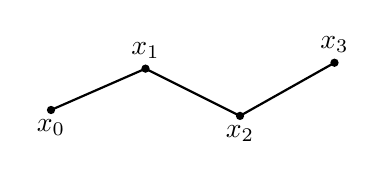
\begin{tikzpicture}[scale=0.75]
\coordinate (x0) at (0,0);\coordinate (x1) at (1.6,0.7);\coordinate (x2) at (3.2,-0.1);\coordinate (x3) at (4.8,0.8);
\draw[thick] (x0)--(x1)--(x2)--(x3);
\foreach \p/\pos/\l in {x0/below/x_0,x1/above/x_1,x2/below/x_2,x3/above/x_3} \fill (\p) circle (2pt) node[\pos]{\(\l\)};
\end{tikzpicture}
\end{column}
\end{columns}
\par
\textbf{The minimal resolution.}
\[
0\longrightarrow S(-3)^{2}\longrightarrow S(-2)^{3}\xrightarrow{\ (m_1,m_2,m_3)\ }S\longrightarrow S/I\longrightarrow0
\]
\textbf{A relation} is an element \((r_1,r_2,r_3)\) of the kernel of \(S(-2)^3\to S\). For example
\[
\underbrace{x_3}_{r_1}\,m_1\ +\ \underbrace{(-x_2)}_{r_2}\,m_2\ +\ \underbrace{0}_{r_3}\cdot m_3\ =\ 0.
\]
\textbf{The other relation.} \(r=(0,\,x_1,\,-x_0)\). The two generate all relations.
\end{frame}

\begin{frame}{The criterion in the example}
\textbf{The relation.}
\[
\underbrace{x_3}_{r_1}\,m_1\ +\ \underbrace{(-x_2)}_{r_2}\,m_2\ +\ \underbrace{0}_{r_3}\cdot m_3\ =\ 0.
\]
\textbf{A choice.} \(H=(x_1^2,\,0,\,0)\): only \(m_1\) changes, to \(m_1+t\,x_1^2\). With the same \(r_i\) we do not get \(0\):
\[
x_3\,(m_1+t\,x_1^2)\ +\ (-x_2)\,m_2\ +\ 0\cdot m_3\ =\ t\,x_1^2x_3\ =\ t\,x_1\cdot m_3.
\]
\textbf{The deformed relation.} What is left is a multiple of \(m_3\). Move it to the left side:
\[
\underbrace{x_3}_{r_1+t\,r_1'}\,(m_1+t\,x_1^2)\ +\ \underbrace{(-x_2)}_{r_2+t\,r_2'}\,m_2\ +\ \underbrace{(0-t\,x_1)}_{r_3+t\,r_3'}\,m_3\ =\ 0.
\]
So \(r'=(0,\,0,\,-x_1)\): the criterion holds for this relation.
\par
\textbf{The other relation} has no \(m_1\): it still holds, with \(r'=0\). So the deformation is flat. It leads to the twisted cubic.
\end{frame}

\begin{frame}{Why the average is an extension}
\small
\textbf{What is obvious.} Each \(\gamma\cdot D_{n+1}\) has equations \(F_i+t^{n+1}(\text{new terms})\). The average still reduces to \(D_n\), and it is \(G\)-equivariant, because \(G\) permutes the six.
\par
\textbf{What is hidden.} An extension is a \emph{flat} deformation, not just sixteen equations. So the claim is: an average of flat ones is flat. A sum of two is not.
\par
\textbf{Why averages work.} Flatness of \(F_i+t^{n+1}A_i\) is a linear condition on the new terms \(A_i\), with a constant term. For each relation \(r\) among the \(m_i\) it reads
\[
\boxed{c(r)+\sum_i r_iA_i\in I,}
\]
where \(c(r)\) is the residue that \(D_n\) leaves on that relation. It does not depend on \(A\).
\begin{itemize}
\setlength{\itemsep}{1pt}
\item If \(A\) and \(B\) satisfy it, so does \(\frac12(A+B)\): \(c(r)\) appears once, as it should.
\item \(A+B\) does not: \(c(r)\) would appear twice.
\end{itemize}
\textbf{Compare.} At first order the condition is \(\sum r_iH_i\in I\), with no constant term: there, sums are allowed. And \(o(D_n)=0\) says that the condition has a solution at all.
\src{\textcolor{red}{The linear condition: derived for this slide, no source checked.}}
\end{frame}

\begin{frame}{All the simple maps}
\small
\textbf{The same question for every fraction.} We just saw that the simple map of \(ce/bf\) is flat. Each fraction \(p/q\) gives a simple map. Which of them are flat?
\par
\textbf{The count,} checking the pair relations in the same way:
\begin{itemize}
\setlength{\itemsep}{1pt}
\item \(109\) fractions give a flat simple map with at least one nonzero correction;
\item \(56\) of them are \(x_i/x_j\): the change of coordinates \(x_j\mapsto x_j+t\,x_i\). These change nothing;
\item \(53\) remain. \(G\) permutes them, in ten orbits, of sizes \(6,6,6,6,6,6,6,6,3,2\).
\end{itemize}
\textbf{One fraction from each orbit.} The first is our example.
\[
\frac{ce}{bf},\ \ \frac{ce}{af},\ \ \frac{c^2e}{abf},\ \ \frac{ce^2}{abf},\ \ \frac{ce}{ab},\ \ \frac{df}{cg},\ \ \frac{d^2f}{acg},\ \ \frac{fh}{ab},\ \ \frac{ef}{ab},\ \ \frac{ac}{bf}.
\]
\textbf{Why this matters.} The \(53\) are a basis of \(T^1\). So, up to changes of coordinates, a \(G\)-equivariant first-order deformation is \(c_1R_1+\cdots+c_{10}R_{10}\), with \(R_k\) the sum over the \(k\)-th orbit. There is nothing else to choose: only the ten numbers \(c_k\).
\src{The count: a script written for this slide. \textcolor{red}{That the \(53\) are a basis of \(T^1\): not re-checked.}}
\end{frame}

\begin{frame}{The \(56\): changes of coordinates}
\textbf{The fraction \(d/a\).} Its simple map replaces \(a\) by \(d\) in the six cubics that contain \(a\):
\[
\begin{array}{llll}
abf\mapsto bdf\in I,&\quad abg\mapsto bdg\in I,&\quad abh\mapsto bdh,\\[2pt]
acg\mapsto cdg,&\quad ach\mapsto cdh,&\quad adh\mapsto d^2h.
\end{array}
\]
So four cubics change: \(\ abh+t\,bdh,\quad acg+t\,cdg,\quad ach+t\,cdh,\quad adh+t\,d^2h\).
\par
\textbf{The same thing, by a substitution.} Put \(a+t\,d\) in place of \(a\) in all sixteen cubics, and remember \(t^2=0\):
\[
(a+t\,d)\,bh=abh+t\,bdh,\qquad(a+t\,d)\,dh=adh+t\,d^2h,\qquad\dots
\]
The cubics without \(a\) do not change. We get exactly the equations above (and \(abf+t\,bdf\), \(abg+t\,bdg\), which give the same ideal).
\par
\textbf{So nothing happened.} The new equations are the old ones in the coordinates \(a'=a+t\,d\). The scheme is \(\SR(\mathcal M)\), moved by a linear change of coordinates of \(\Pj^7\). Flat for free, and not a new deformation.
\par
\textbf{In general.} The fraction \(x_i/x_j\) is the substitution \(x_j\mapsto x_j+t\,x_i\). There are \(8\cdot7=56\) of them.
\end{frame}

\begin{frame}{Our first-order deformation is flat and \(G\)-equivariant}
\textbf{Row by row.} Moving a row by \(G\) and adding gives a deformation that is flat and \(G\)-equivariant: this was shown two slides ago for the first row, and the argument for \(G\)-equivariance is the same for every row. Flat: each simple map passes the criterion, by dividing monomials. \textcolor{red}{We did this by hand only for the first row.}
\par\medskip
\textbf{Sums.} Both properties pass to sums and to multiples:
\begin{itemize}
\setlength{\itemsep}{2pt}
\item the criterion asks that \(\sum r_iH_i\) be in \(I\), and \(I\) is closed under sums;
\item if \(\delta\in G\) permutes the equations \(m_i+tH_i\) and the equations \(m_i+tH_i'\) in the same way as it permutes the \(m_i\), it permutes the equations \(m_i+t\,(H_i+H_i')\).
\end{itemize}
\textbf{So} \(m_i+tH_i\) is a \(G\)-equivariant first-order deformation: this is our \(D_1\). It extends to a flat \(G\)-equivariant family over \(\operatorname{Spec}\C[[t]]\).
\par\medskip
\textbf{Two of the sixteen, in full.}
\[
H_1=ace+2\,bce+3\,c^2e+4\,ce^2+5\,cef+8\,f^2h+9\,ef^2+10\,a^2c,\qquad H_7=10\,acd+10\,cfg.
\]
\src{Checked for this slide by a script: the \(H_i\) built from the table pass the criterion for all \(120\) pairs of cubics, and each element of \(G\) permutes the sixteen equations.}
\end{frame}

\begin{frame}{What is the map in a simple map?}
It is a function between modules. Put \(S=\mathbb C[a,\ldots,h]\)
and let \(I\) be the ideal generated by our sixteen cubics.
The map we want is
\[
\varphi:I\longrightarrow S/I.
\]
Its input is a polynomial in \(I\). Its output is its correction,
read modulo \(I\). For the example \(abf\mapsto abf+t\,ace\) we prescribe
\[
\varphi(abf)=ace\bmod I,\qquad
\varphi(m_i)=0\quad\text{for every other generator}.
\]
We extend by \(S\)-linearity. For instance,
\(\varphi(g\cdot abf)=g\cdot\varphi(abf)\).
Since \(g\cdot abf=f\cdot abg\), these inputs must have the same
output. They do: \(g\cdot ace=e\cdot acg\) is zero in \(S/I\).
Checking all generator relations makes the function well defined.
\end{frame}

\begin{frame}{First-order deformations are maps \(I\to R\)}
\textbf{Notation.} \(S=\C[a,\dots,h]\), \(I=I_{\mathcal M}=(m_1,\dots,m_{16})\), \(R=S/I\).
\par
\textbf{The minimal resolution of \(R\).}
\[
0\longrightarrow S(-8)\longrightarrow S(-5)^{16}\longrightarrow S(-4)^{30}\longrightarrow S(-3)^{16}\xrightarrow{\ (m_1,\dots,m_{16})\ }S\longrightarrow R\longrightarrow0
\]
\textbf{A relation} is an element of the kernel of the map \(S(-3)^{16}\to S\): a row \((r_1,\dots,r_{16})\) of polynomials with \(\sum r_im_i=0\).
\par
\textbf{What we saw.} The criterion: for every relation \(\sum r_im_i=0\) there are \(r_i'\) with \(\sum(r_i+t\,r_i')(m_i+tH_i)=0\). Since \(t^2=0\), the left side is \(t\,\bigl(\sum r_iH_i+\sum r_i'm_i\bigr)\). So the criterion says: the \emph{residue} \(\sum r_iH_i\) of each relation is in \(I\), that is, \(0\) in \(R\).
\par
\textbf{Said with a map.} This is the condition for the rule \(m_i\mapsto H_i\) (taken in \(R\)) to define an \(S\)-linear map \(I\to R\). So these \(H\) form the vector space \(\operatorname{Hom}_S(I,R)_0\) (the \(0\): cubics go to cubics).
\end{frame}

\begin{frame}{The space \(T^1\)}
\textbf{The maps.} First-order deformations of the sixteen equations: \(\operatorname{Hom}_S(I,R)_0\) (last slide).
\par\medskip
\textbf{Some of them do nothing.} A change of coordinates \(x_j\mapsto x_j+t\,\ell_j\), with \(\ell_j\) linear forms, gives
\[
H_i=\sum_j\ell_j\,\frac{\partial m_i}{\partial x_j}.
\]
The scheme is the same, in other coordinates.
\par\medskip
\textbf{Definition.}
\[
\boxed{T^1=\frac{\operatorname{Hom}_S(I,R)_0}{\text{the maps that come from a change of coordinates}}}
\]
Its elements: first-order deformations of \(\SR(\mathcal M)\), up to change of coordinates.
\end{frame}

\begin{frame}{The space \(T^2\)}
\textbf{Relations.} A relation is a row \(r=(r_1,\dots,r_{16})\) of polynomials with \(\sum r_im_i=0\). They form \(\mathrm{Rel}\).
\par
\textbf{Koszul relations.} \(m_j\cdot m_i-m_i\cdot m_j=0\): they exist for any list of polynomials. They generate \(K\subset\mathrm{Rel}\).
\par
\textbf{Residues.} An \(S\)-linear map \(\mathrm{Rel}/K\to R\): it assigns to each relation a residue in \(R\). A row of cubics \(h=(h_1,\dots,h_{16})\) gives such a map: \(r\mapsto\sum r_ih_i\).
\par
\textbf{Definition.}
\[
\boxed{T^2=\frac{\operatorname{Hom}_R(\mathrm{Rel}/K,\,R)_0}{\text{the maps that come from a row of cubics}}}
\]
\textbf{In words.} Residues of the relations, modulo those that a change of equations removes. \textbf{For \(\mathcal M\):} \(\dim T^2=27\).
\src{Heap Project, chapter Deformations, section ``Cotangent obstructions and the Grünbaum quadrics'': the definition of \(T^2_{A,0}\), after Fausk and Hartshorne. \textcolor{red}{Not re-checked for this slide.}}
\end{frame}

\begin{frame}{The obstruction}
\textbf{A deformation of order \(n\).} A deformation of \(\SR(\mathcal M)\) with \(B=\operatorname{Spec}\C[t]/(t^{n+1})\), given by equations \(F_i=m_i+tH_i+\cdots+t^nF_{i,n}\). Call it \(D_n\).
\par
\textbf{Wanted.} A \(D_{n+1}\) that extends it: one more term \(t^{n+1}F_{i,n+1}\) in each equation.
\par
\textbf{What can go wrong.} Each relation among the \(F_i\) holds when \(t^{n+1}=0\). When only \(t^{n+2}=0\), it leaves a residue: \(t^{n+1}\) times a polynomial. So \(D_n\) assigns a residue to each relation. New terms \(F_{i,n+1}\) change the residues by a row of cubics, as on the last slide.
\par
\textbf{The obstruction.} The residues of \(D_n\), modulo the rows of cubics, are one element \(o(D_n)\in T^2\).
\par
\textbf{Theorem.}
\[
\boxed{D_n\text{ extends to some }D_{n+1}\iff o(D_n)=0.}
\]
\textbf{We do not compute \(o(D_n)\):} we show that it lies in a subspace of \(T^2\) which is zero.
\src{Heap Project, chapter Deformations: theorem ``Obstruction to a flat lift'' (Hartshorne, \emph{Lectures on Deformation Theory}, Theorem 10.1). Stacks Project, Tag 08SP. \textcolor{red}{Not re-checked for this slide.}}
\end{frame}

\begin{frame}[allowframebreaks]{References}
\printbibliography[heading=none]
\end{frame}
\end{document}
